\documentclass[fleqn,10pt]{wlscirep}
\usepackage[utf8]{inputenc}
\usepackage[T1]{fontenc}
\usepackage{lineno}
\graphicspath{{./img/}{./pictures/}{./images/}}
\linenumbers

\usepackage[dvipsnames]{xcolor} % colors
\newcommand{\tom}[1]{{\textcolor{RedOrange}{#1}}}
\newcommand{\hh}[1]{{\textcolor{Green}{#1}}}
\usepackage{framed}

\newcommand{\ifinstruction}{0} % 1 for instruction, 0 for no instruction




% for gt tables
%--------------------------------
% gt packages - see gt_latex_dependencies()
\usepackage{booktabs}
\usepackage{caption}
\usepackage{longtable}
\usepackage{colortbl}
\usepackage{array}
\usepackage{anyfontsize}
\usepackage{multirow}
%--------------------------------


% cite-method must be defined in the pre-amble as natbib. 
% any natbib options are overwritten by quarto processing somewhere, so 
% hard code them here
%--------------------------------
\usepackage[super,sort&compress,comma,numbers]{natbib}
%\bibliographystyle{jabbr}
%--------------------------------

\usepackage{subcaption} % for subfigures

\usepackage{float} % for knitr::include_graphics

\title{Three-dimensional data of wire-cut surface scans under the
confocal microscope (110 character maximum, inc. spaces)}

\author[1,2,*]{Yuhang Lin}
\author[2,3]{Heike Hofmann}
\author[4]{Curtis Mosher}
\author[5]{Eden Amin}
\author[2]{Jeff Salyards}
\author[1,2]{Alicia Carriquiry}

\affil[1]{Iowa State University, Department of Statistics, Ames, IA,
50011, USA}
\affil[2]{Iowa State University, Center for Statistics and Applications
in Forensic Evidence (CSAFE), Ames, IA, 50011, USA}
\affil[3]{University of Nebraska-Lincoln, Department of
Statistics, Lincoln, NE, 68583, USA}
\affil[4]{Iowa State University, Roy J Carver High Resolution Microscopy
Facility (HRMF), Ames, IA, 50011, USA}
\affil[5]{University of Central Oklahoma, Criminal Justice and Forensic
Science, Edmond, OK, 73034, USA}

      \affil[*]{corresponding author(s): Yuhang Lin (yhlin@iastate.edu)}
            
\begin{abstract}
\tom{Update later: max of 170 words: describe the study, the assay(s) performed,  resulting data, and reuse potential}

Wire cut data is important in forensic investigations but lacks a
systematic way of analyzing the data. We created a data set of 120 scans
of aluminum wire cut in \texttt{x3p} format, using 5 wire cutters and 3
locations along the 4 blades, with 2 replicates for each combination. A
systematic pipeline with multiple analysis plots was developed to
analyze the data and draw conclusions based on numerical measures.
\end{abstract}
\begin{document}

\flushbottom
\maketitle
%  Click the title above to edit the author information and abstract

\thispagestyle{empty}

\ifnum \ifinstruction=1

\noindent \textcolor{gray}{Please note: Abbreviations should be introduced at the first mention in the main text – no abbreviations lists or tables should be included. Structure of the main text is provided below.}
\fi

\section*{Background \& Summary}\label{sec-background-summary}
\addcontentsline{toc}{section}{Background \& Summary}

An important part of a forensic analysis is the investigation of marks
left at a crime scene. Forensic examiners are in particular interested
in the origin of those marks, ie. in the investigation of their source.
This is known as the Source Identification Problem in Forensic Science
\hh{citation?}. The forensic science community generally distinguishes
between the \textbf{specific source problem}, where the examiner is
interested in whether a mark was left by a specific tool, and
\textbf{the common source problem}, where the focus of the investigation
is on whether two marks were left by the same tool. Current accepted
practice in both of these situations is based on a visual inspection of
the items under a comparison microscope and results, according to the
Theory of Identification \citep{afte} developed by the Association of
Firearm and Toolmark Examiners (AFTE), in a conclusion of the form
\emph{identification} (the marks are believed to have been made by the
same source), \emph{elimination} (the marks on the two items are
believed to have been made by different tools), and \emph{inconclusive}
(there are not enough similiarities or dissimilarities between the marks
to allow either an identification or an elimination). At its core, this
assessment is subjective in its nature and has been criticized in
reports by the National Research Council \citep{nas2009} and the
President's Council of Advisors on Science and Technology \citep{pcast}
for its lack of objectivity and the absence of error rates.

Both of these issues rely on data with known ground-truth.

\hh{Biedermann}\citep{biedermannStrangePersistenceSource2022}
\hh{distinguishes between internal and external perspectives in the forensic literature. The external perspective only allows general statements based on (black-box) studies relating examiners' conclusions to ground truth without considering any evidence of a particular case. To allow an internal perspective, there is a need to quantitatively capture  the basis for an evaluation based on specific evidence.   }

When a bladed tool cuts a wire, striation marks are left on the cut
surface of the wire, as shown in Figure~\ref{fig-cut-microscope}.

\begin{figure}

\centering{

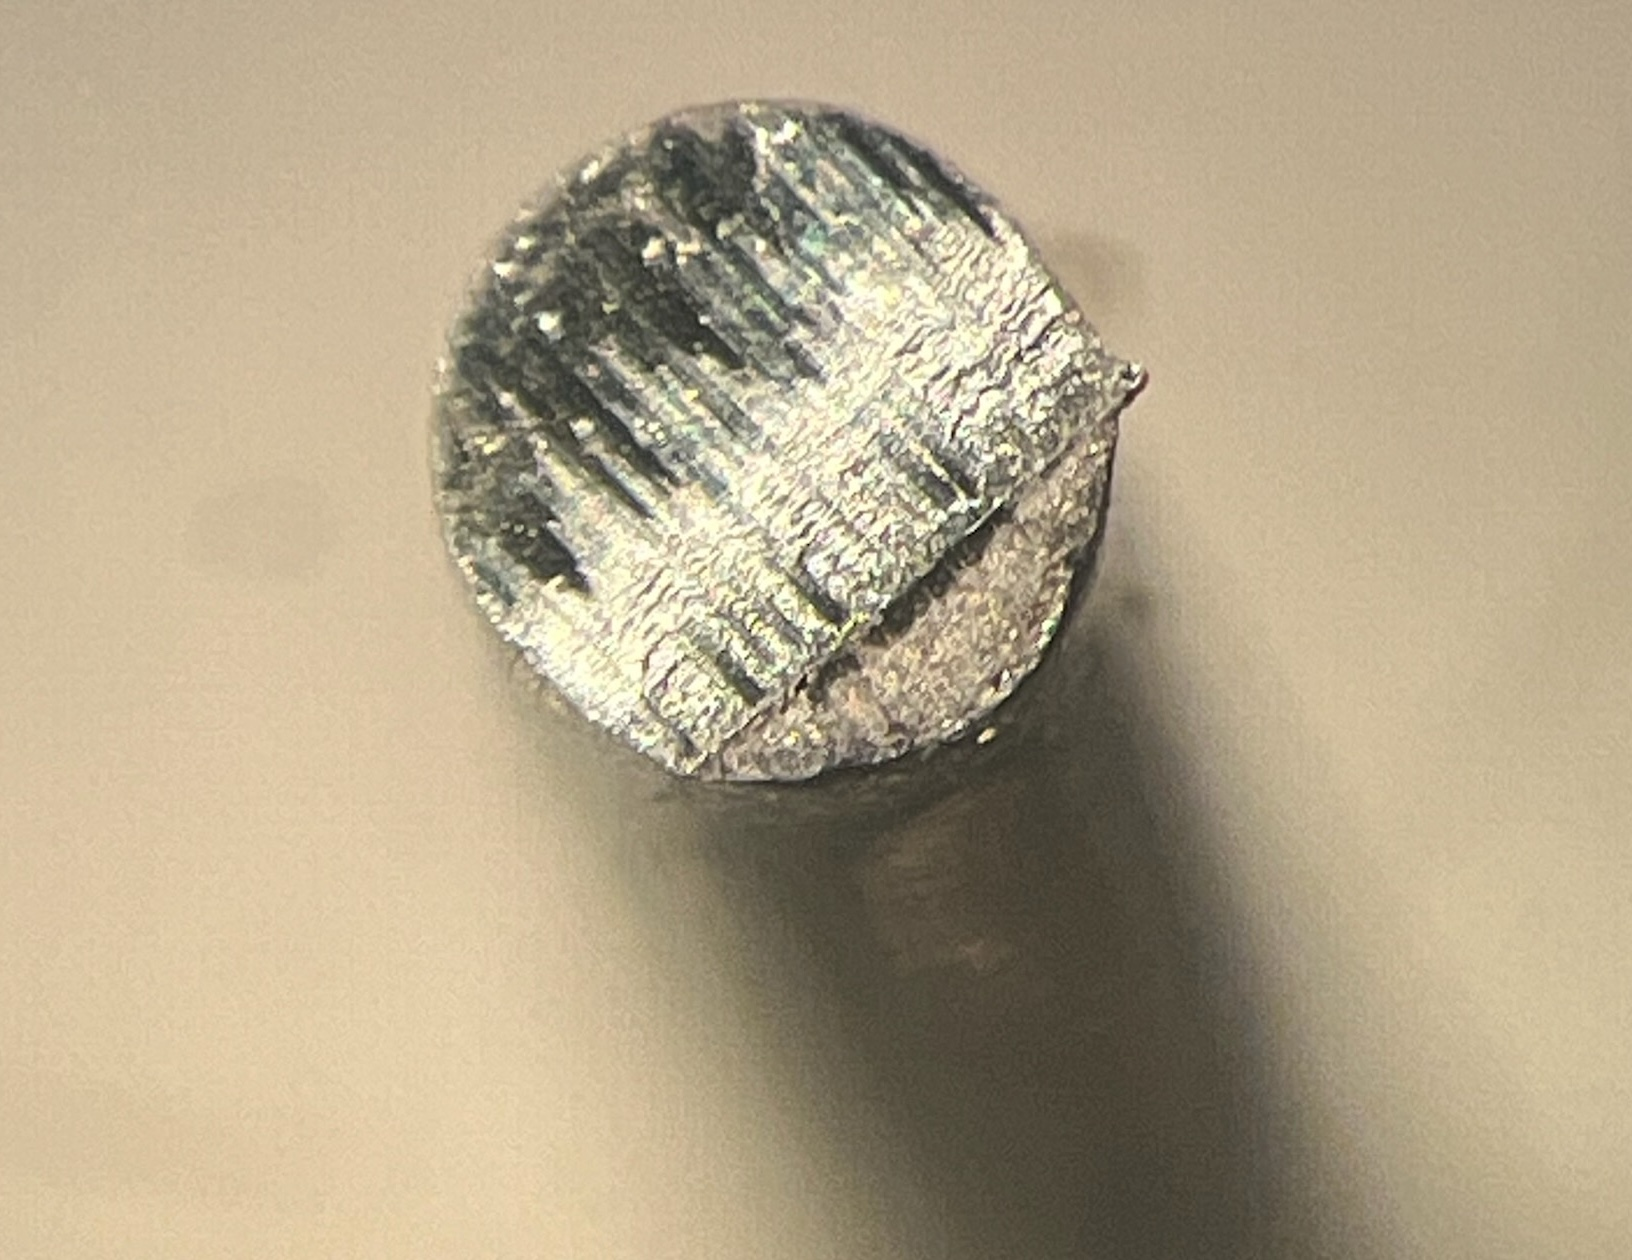
\includegraphics[width=4.16667in,height=3.125in]{images/IMG_72116.jpg}

}

\caption{\label{fig-cut-microscope}Microscopic close-up of striations
left by a blade on the cut end of a wire.}

\end{figure}%

Wire cut data is a type of forensic tool mark data used to assess
similarity of striations left on the surface by a wire cutter. There
have been cases where the evidence and testimony on wire cut evidence
played a crucial role in the criminal investigation and conviction of a
defendant.

However, there is a lack of a standardized method to analyze it, except
for visual comparison.

Work on striations made by
screwdrivers\citep{baikerQuantitativeComparisonStriated2014} identified
angle of attack\citep{baikerToolmarkVariabilityQuality2015a}, rotational
axis\citep{garciaInfluenceAxialRotation2017}, and
direction\citep{cuellarAlgorithmForensicToolmark2024} as the main
factors for comparisons.

Earlier research by Ma et al. \citep{maNISTBulletSignature2004} and
Zheng et al. \citep{zhengNISTBallisticsToolmark2016} has focused on
collecting and distributing datasets for this purpose and providing a
foundation for future advancements in tool mark analysis. Studies such
as those by Chu et al. \citep{chuAutomaticIdentificationBullet2013} and
Vorburger et al.
\citep{vorburgerApplicationsCrosscorrelationFunctions2011} have
demonstrated the efficacy of using numerical methods to improve accuracy
and consistency in tool mark analysis. Hare et al.
\citep{hareAutomaticMatchingBullet2017} and Ju et al.
\citep{juJournalOpenSourceImplementation2022} have explored methods for
quantifying the similarity between representative signals, but alignment
remains a major hurdle.

In this study, we would like to follow the same path and provide a data
set of wire cut scans, and also discuss a systematic pipeline to analyze
the data and draw conclusions based on numerical measures. Here, we
provide a data set containing multiple files, as described in
Table~\ref{tbl-data-overview}.

\begin{table}

\caption{\label{tbl-data-overview}Structure of available data and
files.}

\centering{

\fontsize{12.0pt}{14.4pt}\selectfont
\begin{tabular*}{0.97\linewidth}{@{\extracolsep{\fill}}>{\raggedright\arraybackslash}p{\dimexpr 0.26\linewidth -2\tabcolsep-1.5\arrayrulewidth}|>{\raggedright\arraybackslash}p{\dimexpr 0.56\linewidth -2\tabcolsep-1.5\arrayrulewidth}>{\raggedright\arraybackslash}p{\dimexpr 0.18\linewidth -2\tabcolsep-1.5\arrayrulewidth}}
\toprule
 & Description & Section \\ 
\midrule\addlinespace[2.5pt]
\multicolumn{3}{>{\raggedright\arraybackslash}m{0.97\linewidth}}{Raw data} \\[2.5pt] 
\midrule\addlinespace[2.5pt]
\texttt{scans/} & folder containing 120 topographic 3d scans corresponding to 30 aluminum wire cuts (x3p format) & \protect\hyperref[sec-cutting-wires]{Cutting Wires} \\ 
\texttt{meta.csv} & meta information for each cut with tool, blade, and location information (CSV format) & \protect\hyperref[sec-cutting-wires]{Cutting Wires} \\ 
\midrule\addlinespace[2.5pt]
\multicolumn{3}{>{\raggedright\arraybackslash}m{0.97\linewidth}}{Manual derivatives} \\[2.5pt] 
\midrule\addlinespace[2.5pt]
\texttt{profiles/} & folder of files with manually extracted profiles (CSV format) & \protect\hyperref[sec-extract-profiles]{Extract Profiles} \\ 
\midrule\addlinespace[2.5pt]
\multicolumn{3}{>{\raggedright\arraybackslash}m{0.97\linewidth}}{Computational derivatives in folder 'data-derived/'} \\[2.5pt] 
\midrule\addlinespace[2.5pt]
\texttt{wire-signals} & signals processed from corresponding profile (zipped CSV format) & \protect\hyperref[sec-filtered-signals]{Filtered Signals} \\ 
\texttt{wire\_pairwise\_ccf} & CCF values of all pairwise aligned signals (zipped CSV format) & \protect\hyperref[sec-align-signals]{Align Signals} \\ 
\midrule\addlinespace[2.5pt]
\multicolumn{3}{>{\raggedright\arraybackslash}m{0.97\linewidth}}{Image files} \\[2.5pt] 
\midrule\addlinespace[2.5pt]
\texttt{pngs/} & folder containing pictures of 3d scans of wire cuts (PNG format) & \protect\hyperref[sec-cutting-wires]{Cutting Wires} \\ 
\texttt{profile-images/} & folder containing pictures of profile extracted from wire cuts (PNG format) & \protect\hyperref[sec-extract-profiles]{Extract Profiles} \\ 
\midrule\addlinespace[2.5pt]
\multicolumn{3}{>{\raggedright\arraybackslash}m{0.97\linewidth}}{Visual Inventory in folder 'assessment/analysis-manual/'} \\[2.5pt] 
\midrule\addlinespace[2.5pt]
\texttt{processing-wires} & display of pairwise aligned signals from the same sources (HTML format) & \protect\hyperref[sec-align-signals]{Align Signals} \\ 
\bottomrule
\end{tabular*}

}

\end{table}%

For the reproducibility of all our data and alignment results, we
introduce in detail in \hyperref[sec-cutting-wires]{Cutting Wires}
\tom{hyperlink location incorrect for unnumbered sections}\hh{it seems that the hyperlinks make sure that the section is on the page}
how we cut the wire and collect the 120 scans with 5 tools, in
\hyperref[sec-extract-profiles]{Extract Profiles} how we extract
profiles from the scans, in \hyperref[sec-filtered-signals]{Filtered
Signals} how we filter signals from the profiles, in
\hyperref[sec-align-signals]{Align Signals} how we align signals from
different scans and optimize the alignment with the cross-correlation
function (CCF) values. In \hyperref[sec-data-records]{Data Records}, we
discuss where our data is held. Then, in
\hyperref[sec-technical-validation]{Technical Validation}, a technical
validation was conducted to further compare signals from different
sources also match our assumption, together with visual aids for drawing
conclusions. Finally, in \hyperref[sec-usage-notes]{Usage Notes}, we
provide available codes for creating the data set and conducting
technical validation, as discussed in \hyperref[sec-methods]{Methods}
and \hyperref[sec-technical-validation]{Technical Validation}.
\hyperref[sec-code-availability]{Code availability} discusses where
these codes can be found online. We hope this pipeline developed using
this data set can be further generalized and applied to real crime
scenes to help investigators draw conclusions based on real wire cut
data.

\ifnum \ifinstruction=1

\textcolor{gray}{(unlimited length) An overview of the study design, the assay(s) performed, and the created data, including any background information needed to put this study in the context of previous work and the literature. The section should also briefly outline the broader goals that motivated the creation of this dataset and the potential reuse value. We also encourage authors to include a figure that provides a schematic overview of the study and assay(s) design. The Background \& Summary should not include subheadings. This section and the other main body sections of the manuscript should include citations to the literature as needed.}
\fi

\section*{Methods}\label{sec-methods}
\addcontentsline{toc}{section}{Methods}

In this study, aluminum wire was used to create an optimal scenario
where the most amount of information could be transferred from the tool
to the substrate despite the wire, in some real cases, being made of
lead. The physical property of aluminum wire makes it an excellent
candidate for keeping marks while being relatively easy to bend and
non-toxic.

\subsection*{Cutting Wires}\label{sec-cutting-wires}
\addcontentsline{toc}{subsection}{Cutting Wires}

The aluminum wire used was 16 Gauge/1.5 mm, anodized. In order to cut
the wire, 4-inch pieces were unspooled and cut using Kaiweets wire
cutters, model KWS-105, as shown in Figure~\ref{fig-plier-tip}, for 1
blade location, either inner, middle, or outer, which gives us 1
replicate. Each piece was then cut into half to create 2-inch pieces for
each side, AB and CD, with a sharpie line marking the cut ends, giving
us 4 samples. Then, we can use the standard scanning protocols for the
confocal microscope, shown in Figure Figure~\ref{fig-wire-microscope},
to scan the wire tip surfaces. The scanned surfaces are saved in a
resolution of \(0.645 \mu m \times 0.645 \mu m\) per square pixel in an
\texttt{x3p} file format. Here, we are showing AB and CD sides in
Figure~\ref{fig-T1AW-LI-R2-4edges}, with the back of A being C and the
back of B being D. Both AB and CD sides form tent structures on the tips
of the wire, and we can separate each side of the tent into 2 pieces
along the bending position, resulting in 8 scans. We repeated this
process for all 3 locations along the blade and 5 wire cutters, with 2
replicates for each tool-edge-location combination, resulting in 120
scans. Each piece was labeled with the naming conventions, T(ool)
1/2/3/4/5 (Edge) A/B/C/D W(ire) - L(ocation) I(nner)/M(iddle)/O(uter) -
R(epetition) 1/2, with T1AW-LI-R1 being the piece cut by tool 1 on the A
edge at the inner location for the first repetition.

\begin{figure}

\begin{minipage}{0.30\linewidth}

\centering{

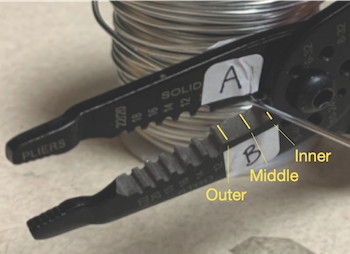
\includegraphics[width=\textwidth,height=0.15\textheight]{images/plier-tip.png}

}

\subcaption{\label{fig-plier-tip}}

\centering{

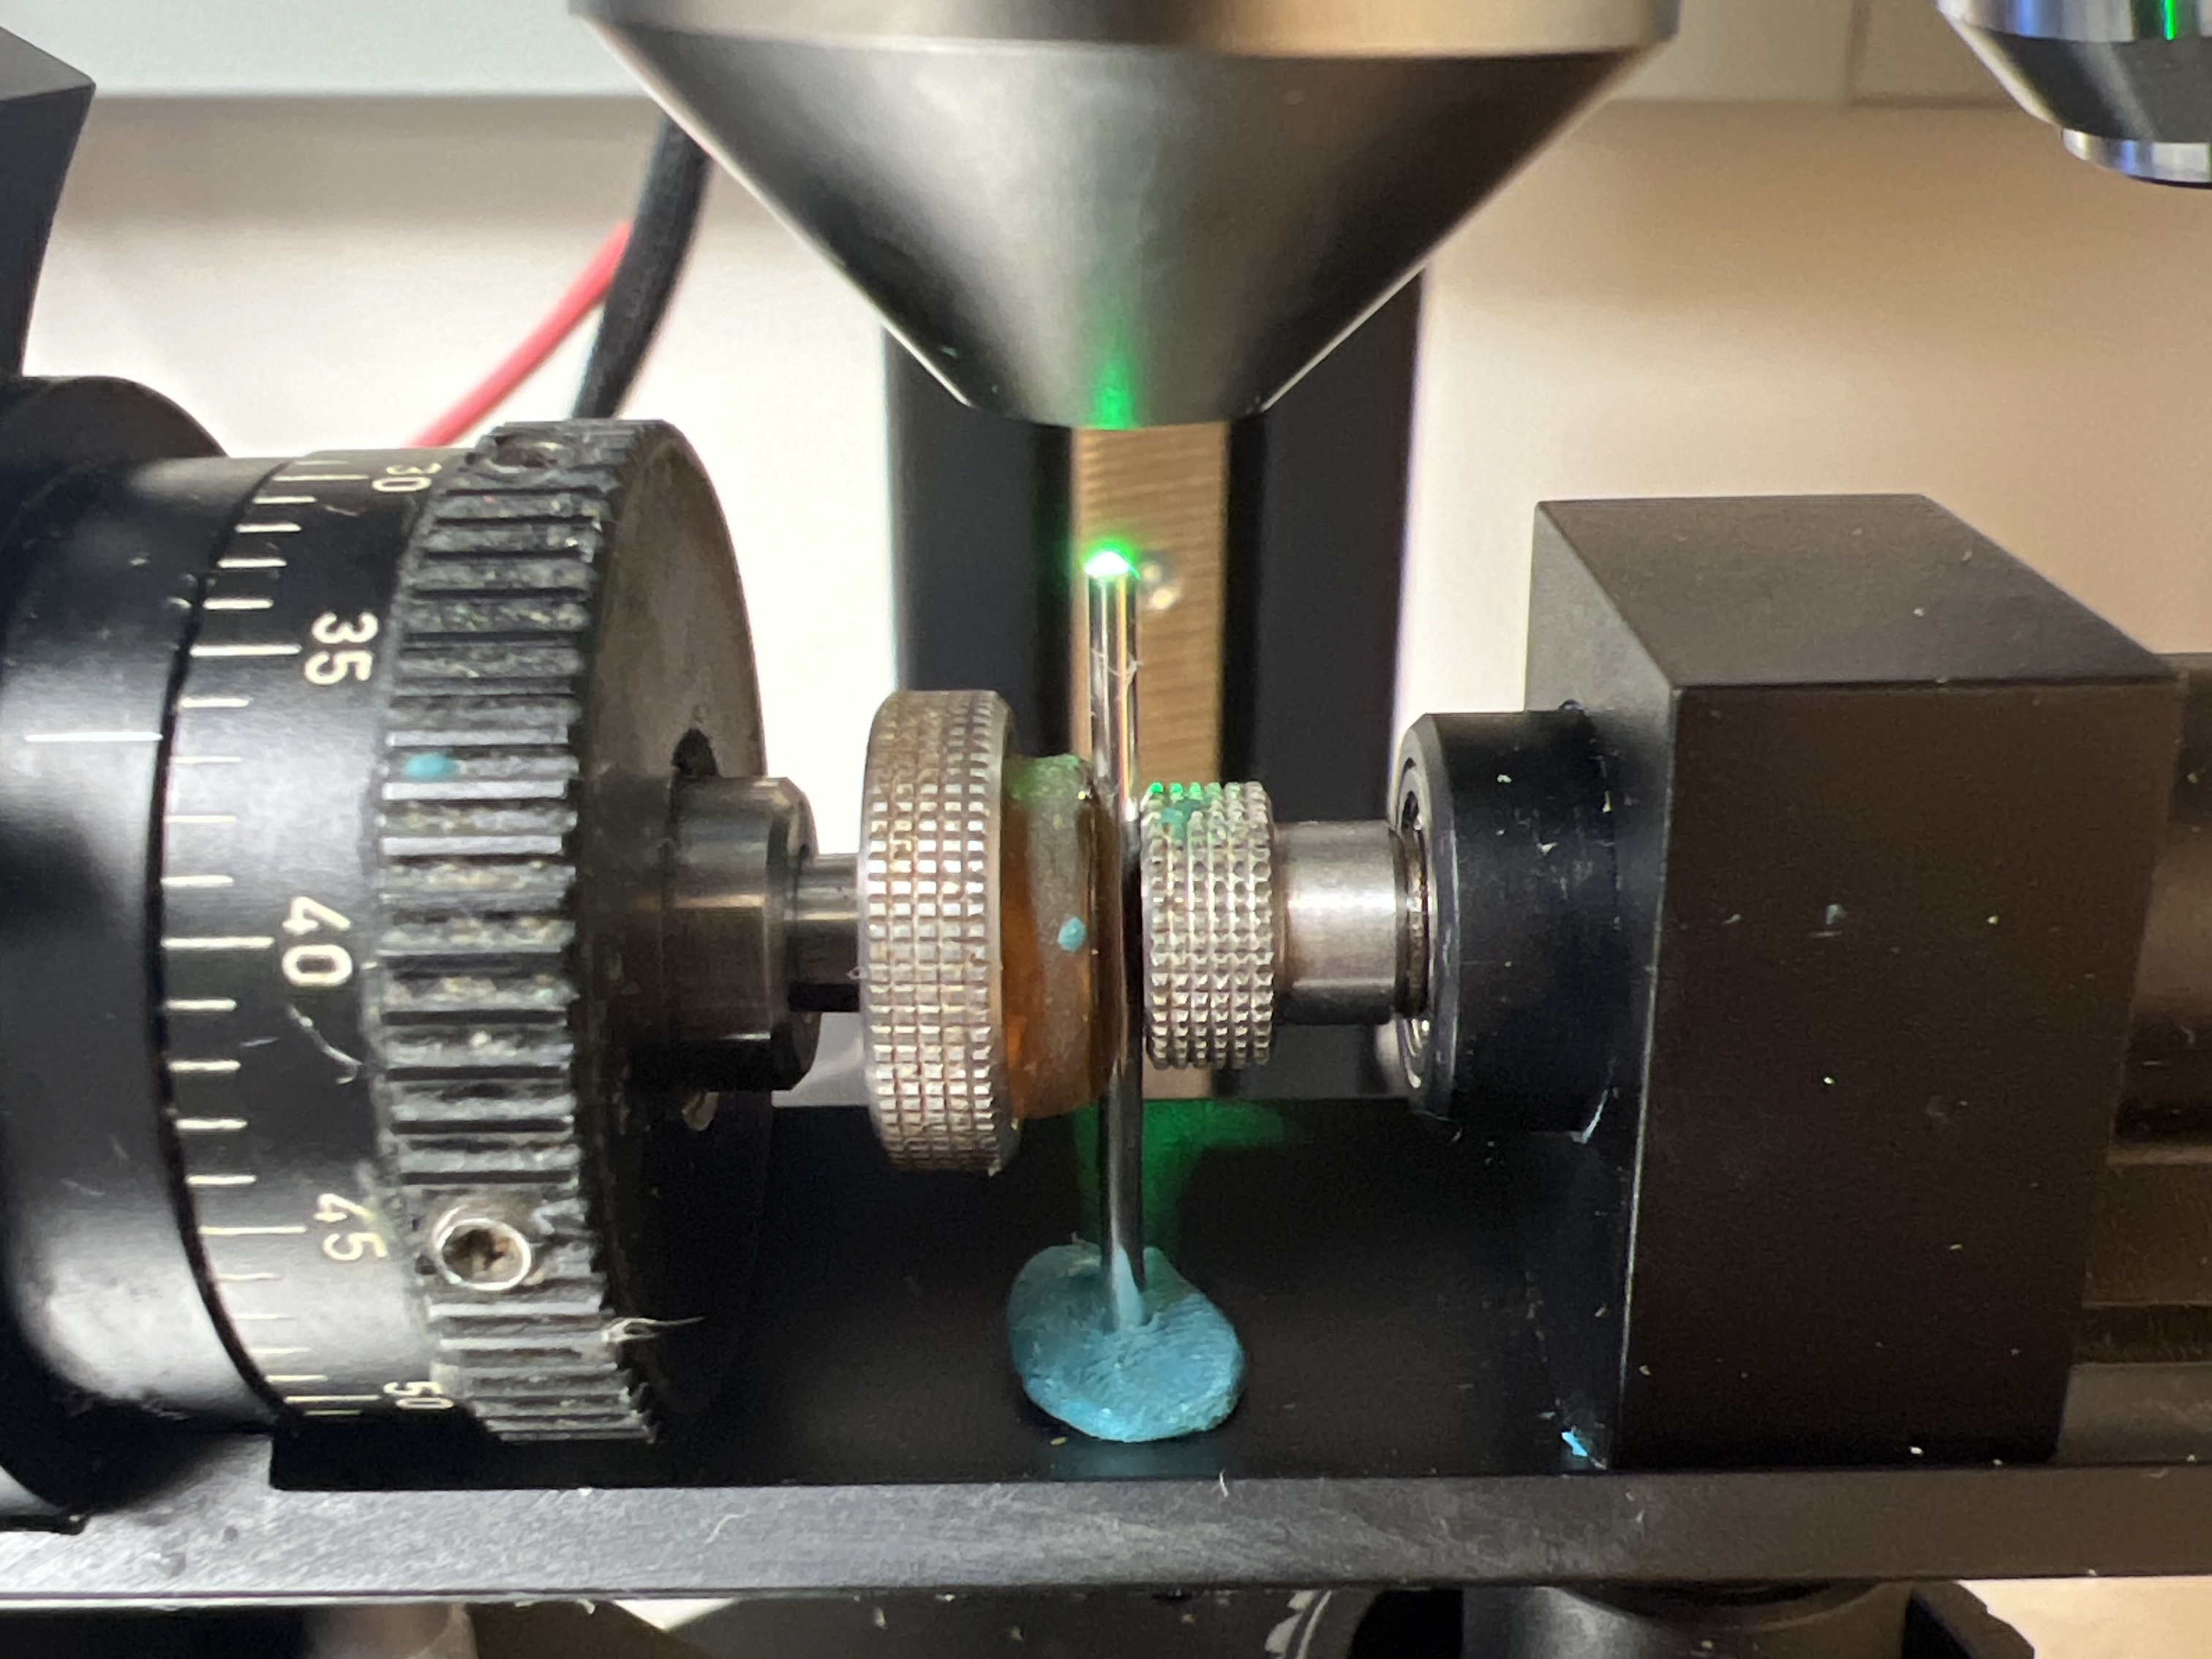
\includegraphics[width=\textwidth,height=0.15\textheight]{images/wire-microscope-062524.JPG}

}

\subcaption{\label{fig-wire-microscope}}

\end{minipage}%
%
\begin{minipage}{0.05\linewidth}
~\end{minipage}%
%
\begin{minipage}{0.65\linewidth}

\centering{

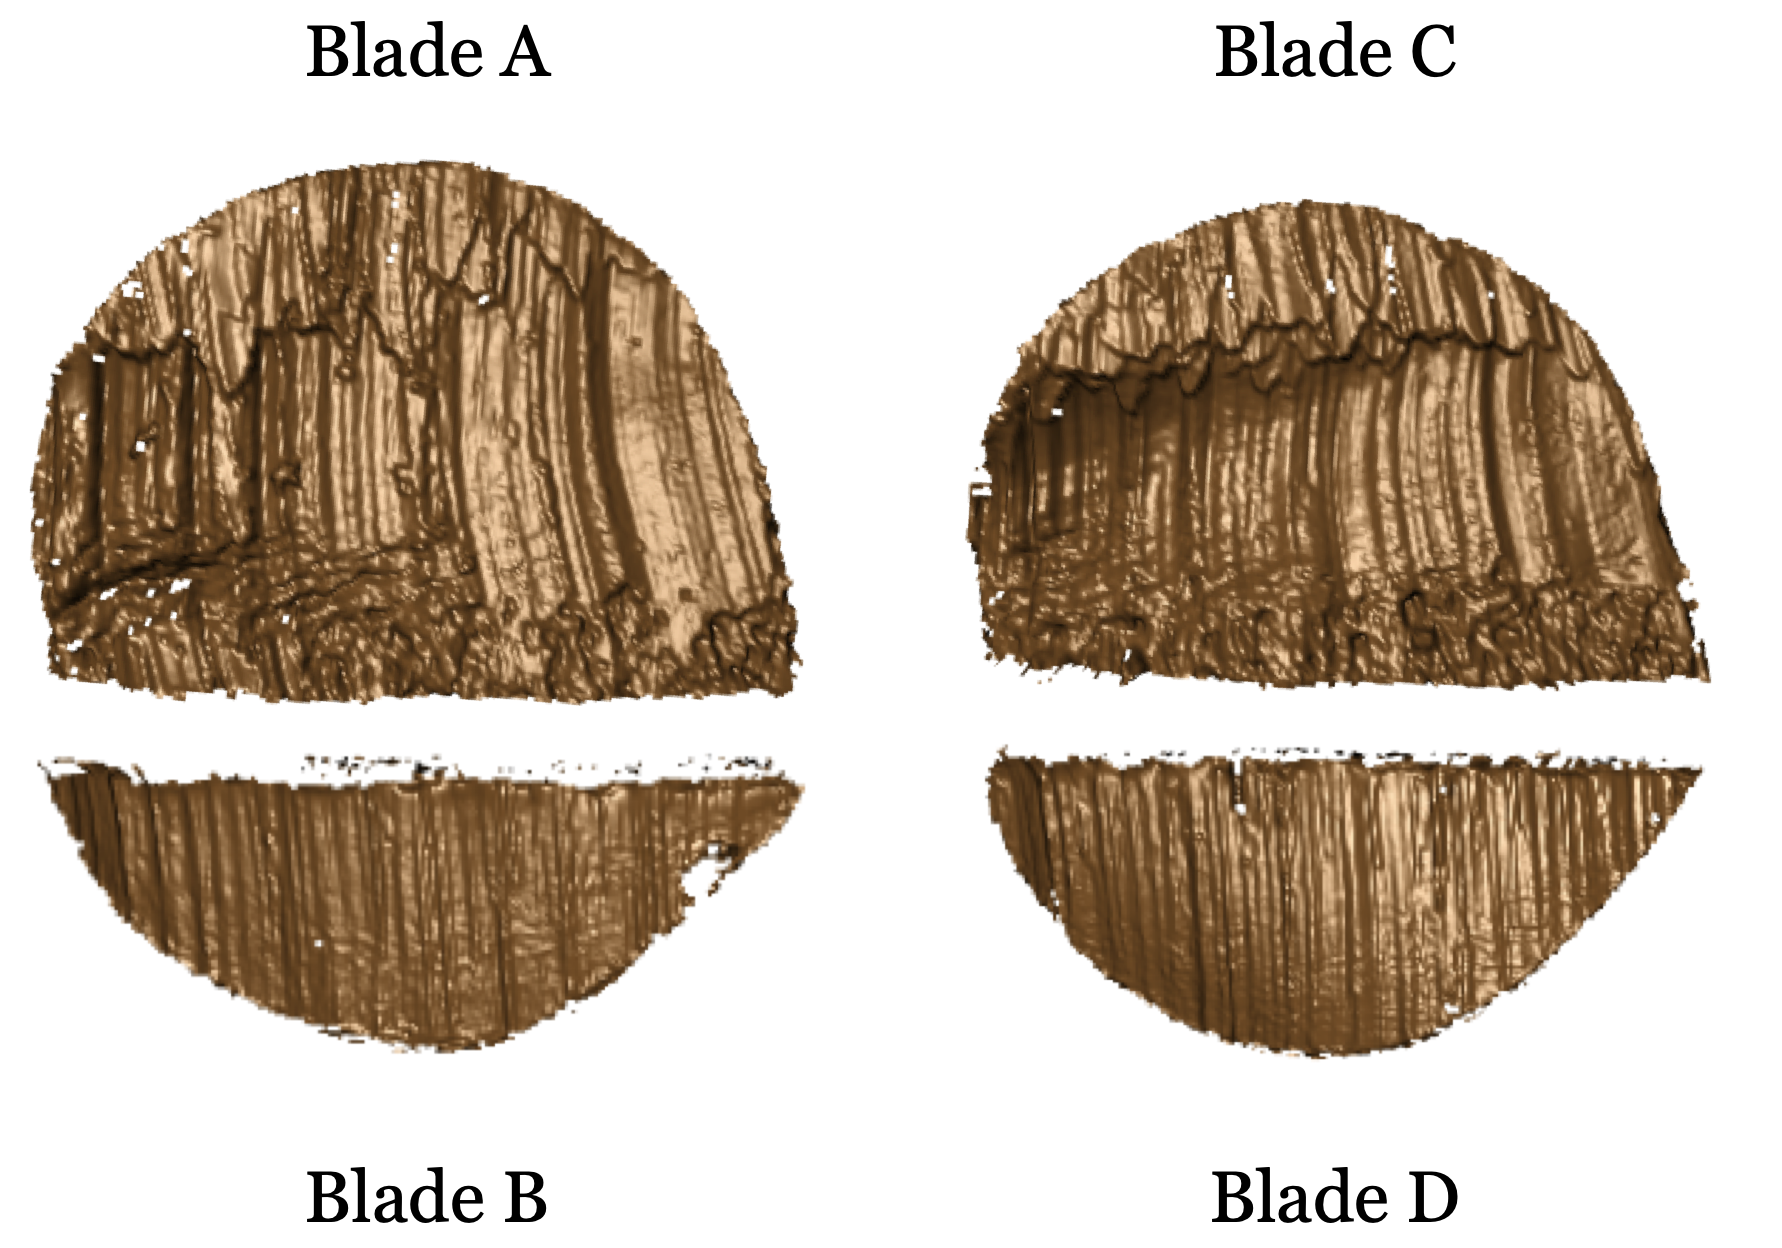
\includegraphics[width=\textwidth,height=0.33\textheight]{images/T1AW-LI-R2-4edges.png}

}

\subcaption{\label{fig-T1AW-LI-R2-4edges}}

\end{minipage}%

\caption{\label{fig-cut-tent-scan}(a) A Kaiweets wire cutter of model
KWS-105 was used to cut the wire, with inner, middle and outer locations
marked. (b) A confocal microscope was used to scan the wire surfaces.
(c) After separating 2 tent structures by the connecting position, we
obtained 4 samples - 2 samples from blade A and B, and others from blade
C and D. \tom{width and height are tuned manually}
\tom{ | full requirements see \href{https://www.nature.com/sdata/publish/submission-guidelines\#figures}{https://www.nature.com/sdata/publish/submission-guidelines\#figures}}}

\end{figure}%

\subsection*{Extract Profiles}\label{sec-extract-profiles}
\addcontentsline{toc}{subsection}{Extract Profiles}

Numerical comparisons between 2 replicates cannot be done directly on
the \texttt{x3p} files. We need to extract representative functions from
the scans first. A representative function with the most information is
considered as a signal for one scan, which can be used later for
comparison. To obtain this function, we first need a profile of the
scan, which is a sequence of values along a user-drawn line on the
surface. The profile should capture most features of the scan and be
orthogonal to the striation marks of the scan, which are formed by the
ups and downs of grooves. So, we draw the line across the wide region of
the scan to maximize the feature captured, as shown in dark blue in
Figure~\ref{fig-T1AW-LI-R1-profiles}. We can then investigate the values
under this profile line. The profile function along the line is plotted
in Figure~\ref{fig-T1AW-LI-R1-profiles-plot}.

\subsection*{Filtered Signals}\label{sec-filtered-signals}
\addcontentsline{toc}{subsection}{Filtered Signals}

With the profile extracted, we can then obtain the signal. Two Gaussian
filters, as discussed in Cleveland et al.
\citep{clevelandLocalRegressionModels1992}, are applied to these
resulting profiles. In particular, we first used a large low-pass filter
with bandwidths of 400 microns to remove the large trend, as it can
overwhelm the signals, and then used a small high-pass filter of 40
microns to average across noise and remove spikes, as shown in
Figure~\ref{fig-T1AW-LI-R1-signals-plot}.
\hh{(add reference: W. S. Cleveland, E. Grosse and W. M. Shyu (1992) Local regression models. Chapter 8 of Statistical Models in S eds J.M. Chambers and T.J. Hastie, Wadsworth \& Brooks/Cole.)}.
Finally, the extreme tail values are removed.

\begin{figure}

\begin{minipage}{0.50\linewidth}

\centering{

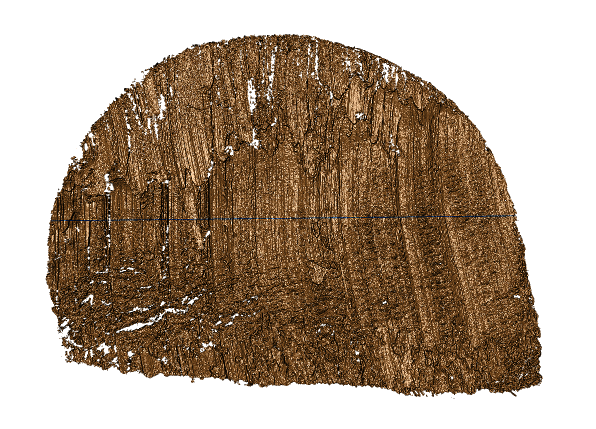
\includegraphics[width=\textwidth,height=0.28\textheight]{images/T1AW-LI-R1-profiles.png}

}

\subcaption{\label{fig-T1AW-LI-R1-profiles}}

\end{minipage}%
%
\begin{minipage}{0.50\linewidth}

\centering{

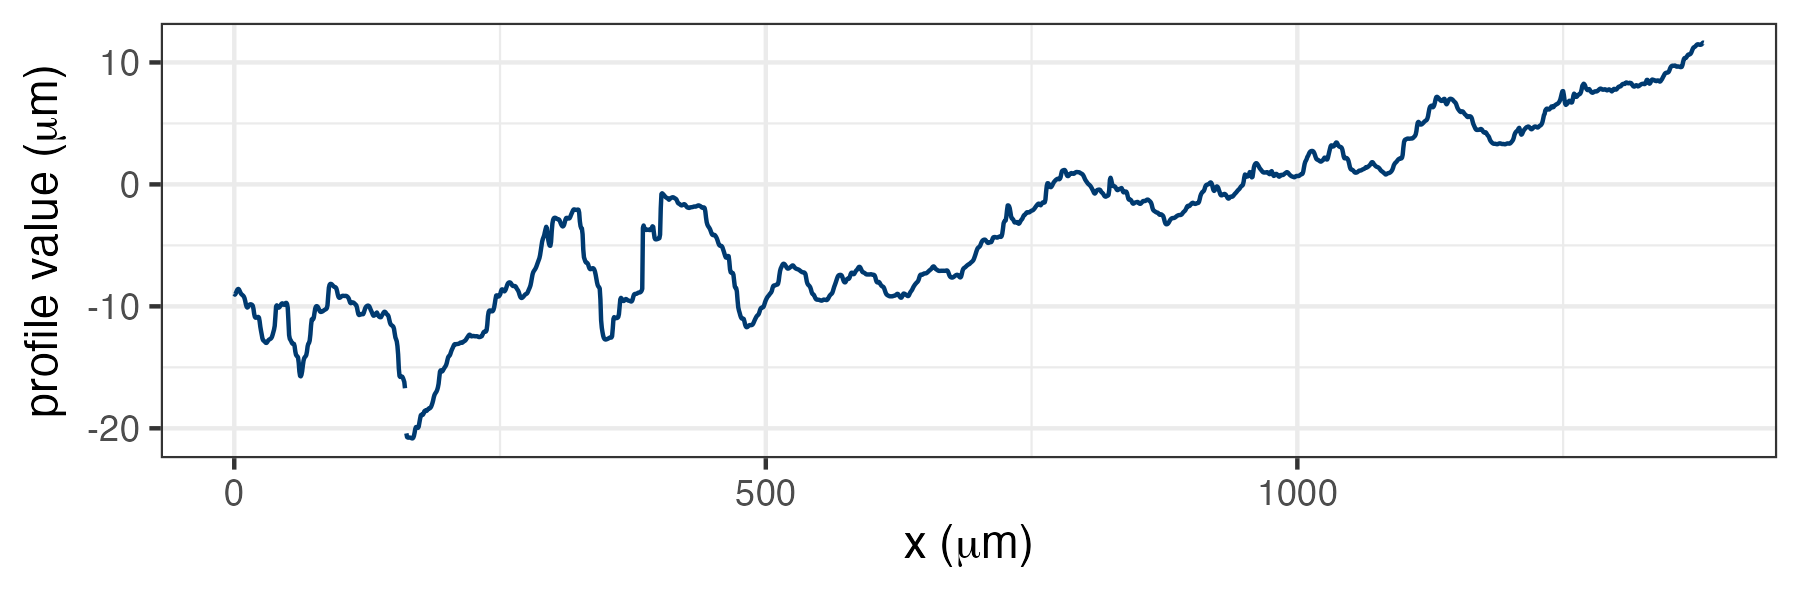
\includegraphics[width=\textwidth,height=0.13\textheight]{images/T1AW-LI-R1-profiles-plot.png}

}

\subcaption{\label{fig-T1AW-LI-R1-profiles-plot}}

\centering{

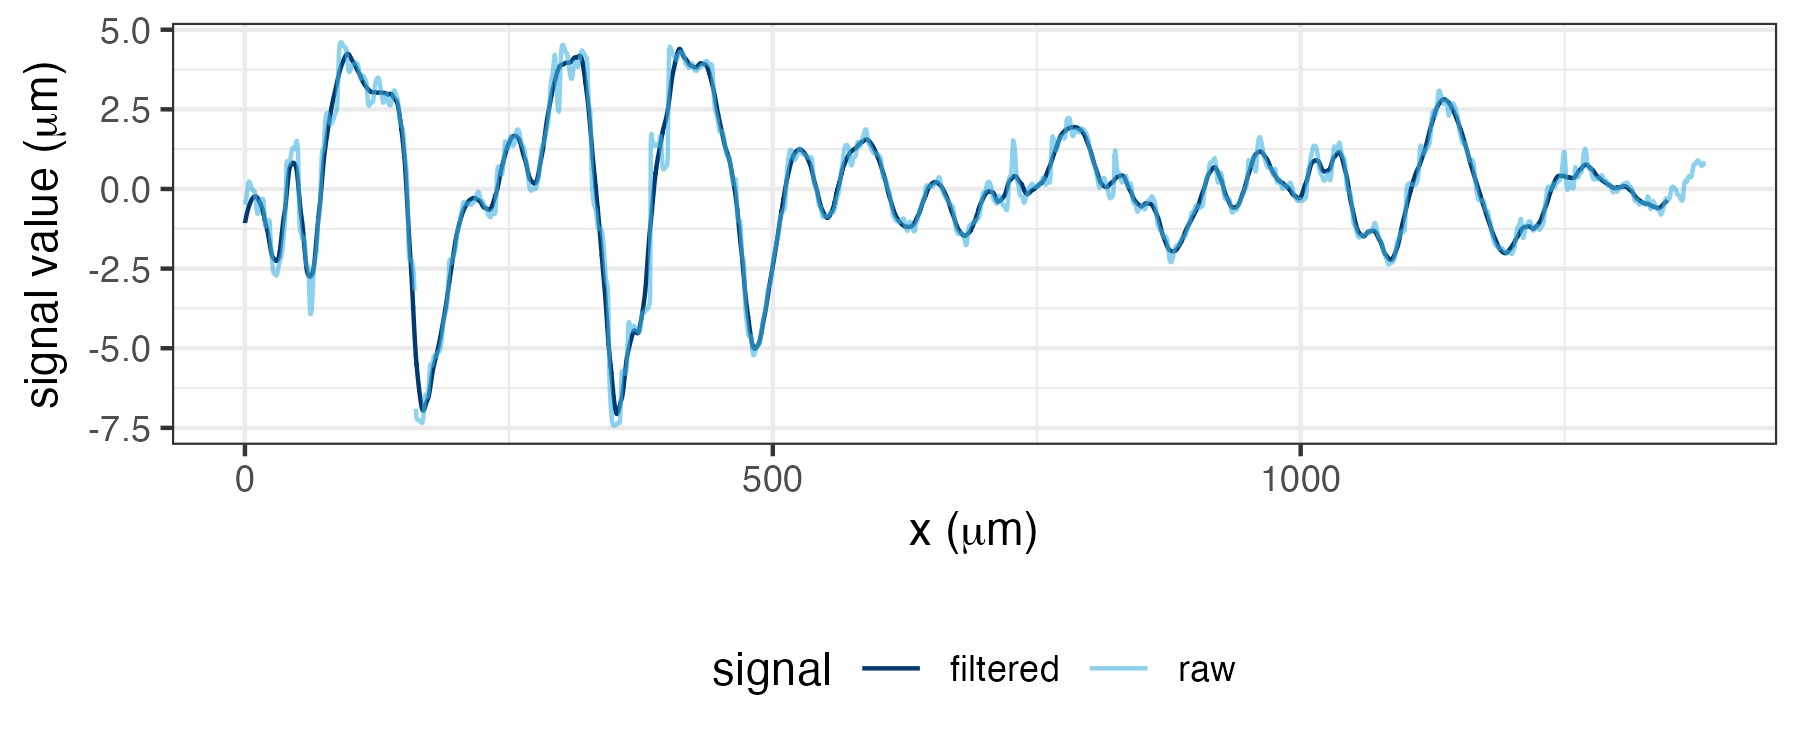
\includegraphics[width=\textwidth,height=0.13\textheight]{images/T1AW-LI-R1-signals-plot.png}

}

\subcaption{\label{fig-T1AW-LI-R1-signals-plot}}

\end{minipage}%

\caption{\label{fig-T1AW-LI-R1-profiles-signals}(a) A profile line in
dark blue was drawn across the striations of the scan. (b) The profile
function extracted along the profile line in (a). (c) The raw signal in
light blue is obtained by using the low-pass filter on the profile
function in (b) and the filtered signal is obtained by using the
high-pass filter on the raw signal.}

\end{figure}%

\subsection*{Align Signals}\label{sec-align-signals}
\addcontentsline{toc}{subsection}{Align Signals}

Signals extracted from different scans can be put together for
comparison, and we maximize the cross-correlation function (CCF) values
between the signals to find the best alignment numerically. For example,
we compare T1AW-LI-R1 to T1AW-LI-R2, T1CW-LI-R1 to T1CW-LI-R2, and so
on. That is comparing each row in Figure \ref{fig-scans-pair}. We know
that signals from two replicates with the same tool-edge-location
combination should yield similar signals, as in the first and second
columns of Figure \ref{fig-signals-pair-alignment}, which will give
alignments of massive overlapping and high CCF values close to 1. The
alignments and values we got in the rightmost column of Figure
\ref{fig-signals-pair-alignment} fulfill our expectations.

\begin{figure}

\centering{

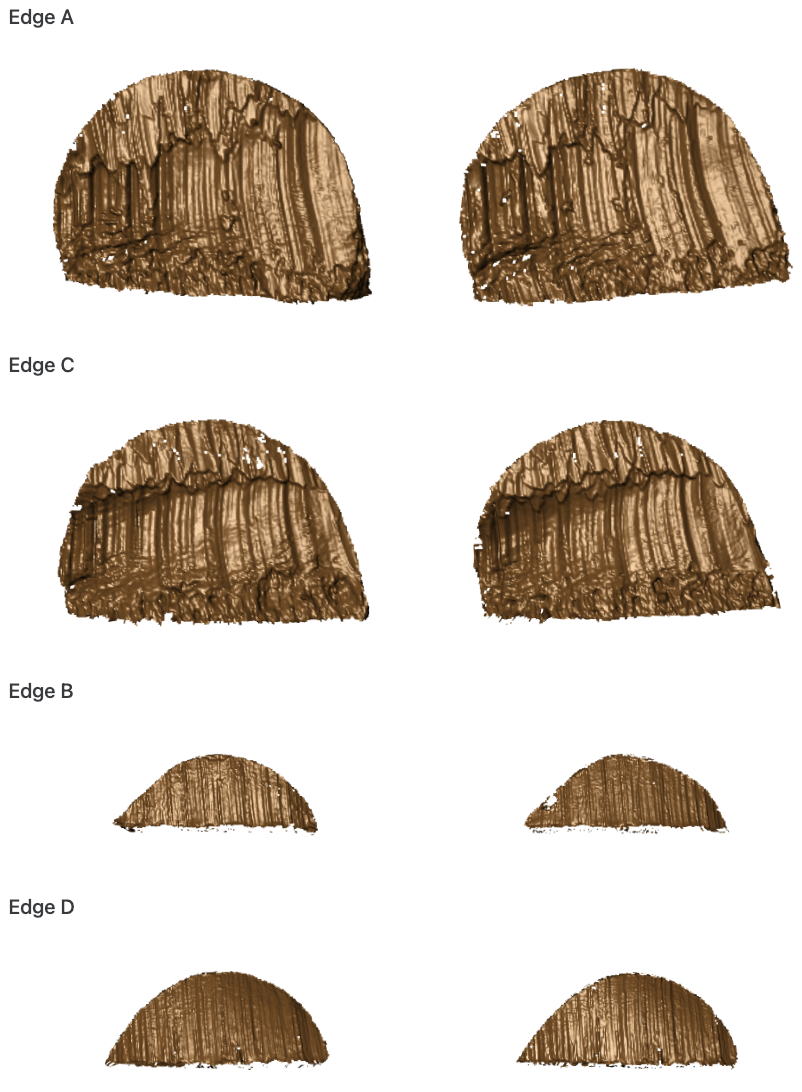
\includegraphics[width=6.25in,height=7.8125in]{images/scans_pair.png}

}

\caption{\label{fig-scans-pair}Scans from different sides of tool 1 at
the inner location.}

\end{figure}%

\begin{figure}

\centering{

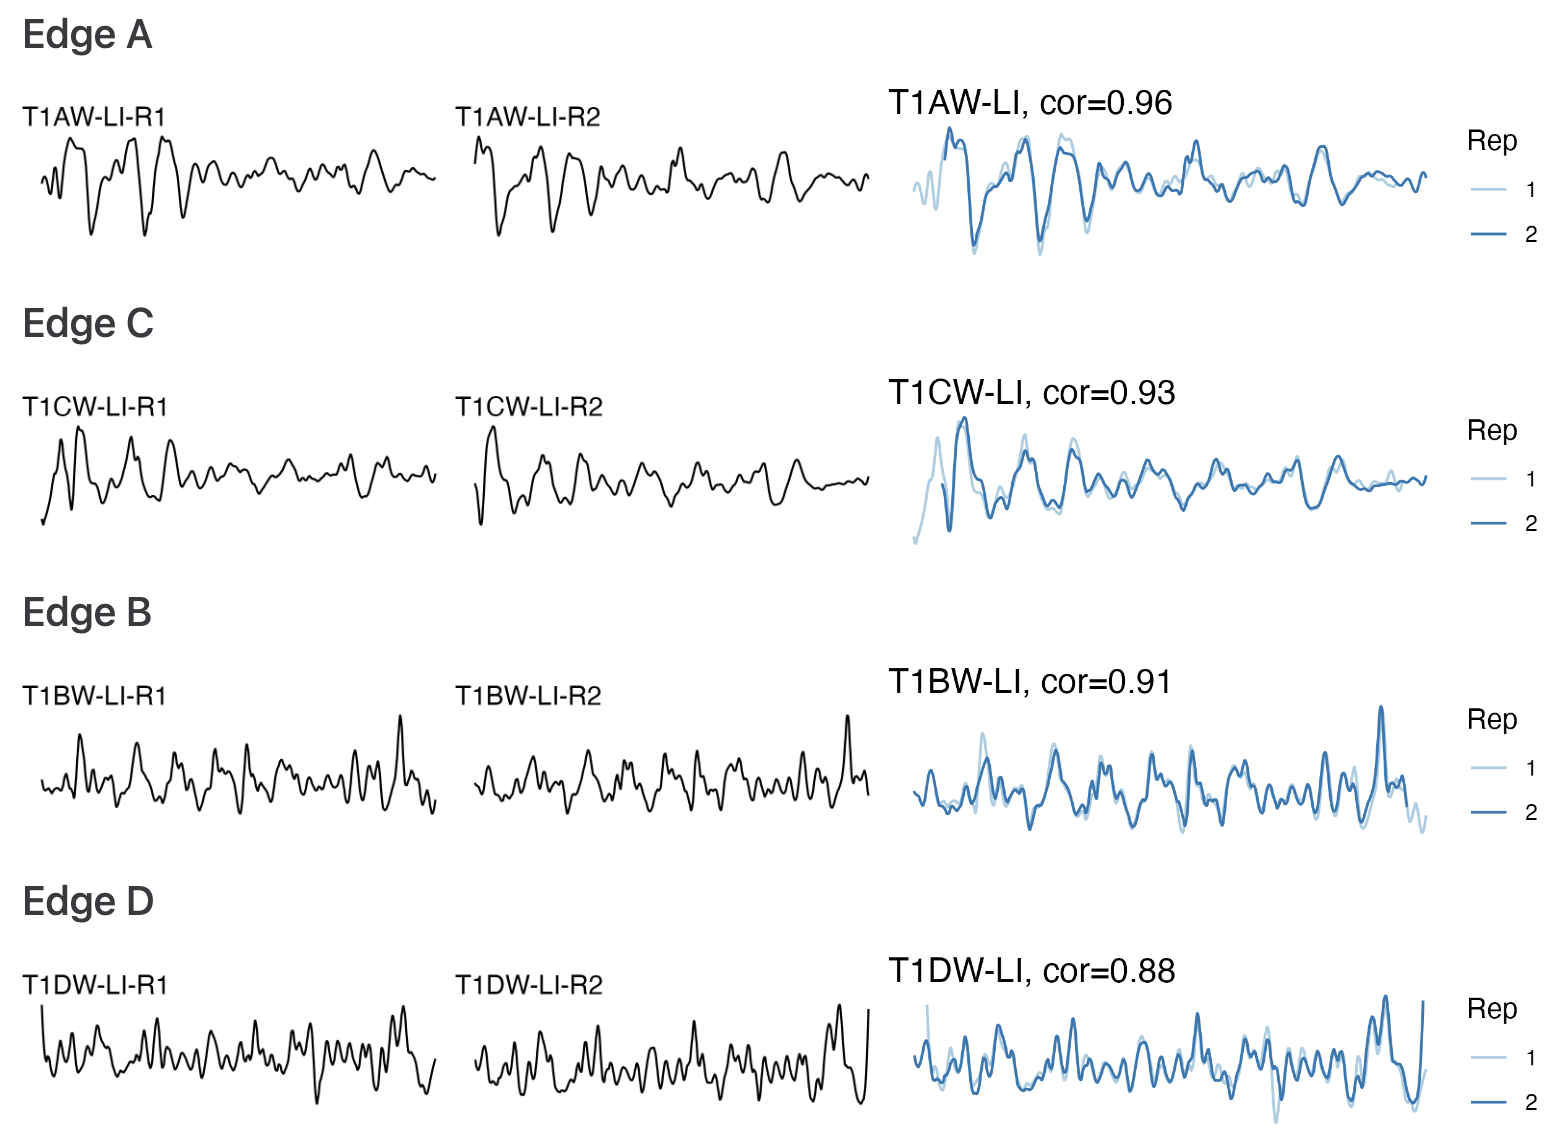
\includegraphics[width=5.20833in,height=3.64583in]{images/signals_pair_alignment.png}

}

\caption{\label{fig-signals-pair-alignment}The first and second columns
show the signals extracted from Figure \ref{fig-scans-pair}, and the
third column shows the alignments and CCF values between pairs of
signals.}

\end{figure}%

\ifnum \ifinstruction=1

\textcolor{gray}{(unlimited length) The Methods should include detailed text describing any steps or procedures used in producing the data, including full descriptions of the experimental design, data acquisition assays, and any computational processing (e.g. normalization, image feature extraction). See the detailed section in our submission guidelines for advice on writing a transparent and reproducible methods section. Related methods should be grouped under corresponding subheadings where possible, and methods should be described in enough detail to allow other researchers to interpret and repeat, if required, the full study. Specific data outputs should be explicitly referenced via data citation (see Data Records and Citing Data, below).}

\textcolor{gray}{Authors should cite previous descriptions of the methods under use, but ideally the method descriptions should be complete enough for others to understand and reproduce the methods and processing steps without referring to associated publications. There is no limit to the length of the Methods section. Subheadings should not be numbered.}

\textcolor{gray}{Authors should review the transparent methods checklist below, and ensure that their manuscript complies with any relevant points. Authors are also encouraged to search FAIRsharing.org for community reporting standards that may be relevant to their specific data-type.}

Transparent Methods Checklist

\begin{itemize}
  \item
  Materials \& reagents:
  Identify commercial suppliers of reagents, instrumentation or kits, when the source is critical to the outcome of the experiments.
  Declare any restrictions on the availability of unique materials (more information here).
  Provide catalogue or clone numbers for all antibodies (if available). For primary antibodies, provide proof of validation for the relevant species and applications.
  
  \item
  Exclusion criteria: If any data or samples were excluded, explain the exclusion criteria and state in the methods whether the criteria were established before the study was conducted.
  
  \item
  Randomization \& blinding: For any studies that involve assigning samples, animals or participants into different groups:
  State clearly whether randomization methods were used. If randomization was not employed, this should be clearly stated.
  State clearly whether blinding was employed during data collection. If blinding was not employed, this should be clearly stated.
  
  \item
  Animal \& human studies (full journal policies here):
  Experiments involving human participants must identify the committee approving the experiments, and include a statement confirming that informed consent was obtained from all participants.
  Studies employing nonhuman animals should ensure that methods descriptions comply with the ARRIVE checklist.
  
  \item
  Cell lines:
  For each eukaryotic cell line used, state the source and whether the cell line has been authenticated or otherwise tested for integrity.
  If any commonly misidentified cell lines were used (see ICLAC or NCBI Biosample), justify their use.
  Report whether the cell lines were tested for mycoplasma contamination.
  
  \item
  Chemistry \& materials science: Manuscripts describing chemical syntheses, or characterizing new chemicals or materials should refer to the guidance at Nature Chemistry.
  
\end{itemize}
\fi

\section*{Data Records}\label{sec-data-records}
\addcontentsline{toc}{section}{Data Records}

The complete data set is available on the ISU DataShare repository at
\href{https://iastate.figshare.com/}{https://iastate.figshare.com/},
which is public and open access for every interested researcher. The
structure of the data set is described before in
Table~\ref{tbl-data-overview}.

\ifnum \ifinstruction=1

\textcolor{gray}{(unlimited length) The Data Records section should be used to explain each data record associated with this work, including the repository where this information is stored, and to provide an overview of the data files and their formats. Each external data record should be cited numerically in the text of this section, for example \cite{Hao:gidmaps:2014}, and included in the main reference list as described below. A data citation should also be placed in the subsection of the Methods containing the data-collection or analytical procedure(s) used to derive the corresponding record. Providing a direct link to the dataset may also be helpful to readers (\hyperlink{https://doi.org/10.6084/m9.figshare.853801}{https://doi.org/10.6084/m9.figshare.853801}).}

\textcolor{gray}{Tables should be used to support the data records, and should clearly indicate the samples and subjects (study inputs), their provenance, and the experimental manipulations performed on each (please see 'Tables' below). They should also specify the data output resulting from each data-collection or analytical step, should these form part of the archived record.}
\fi

\section*{Technical Validation}\label{sec-technical-validation}
\addcontentsline{toc}{section}{Technical Validation}

For the data collection process, two team members did the cutting and
labeling together, then one person did the scanning and named according
to the naming convention introduced in
\hyperref[sec-cutting-wires]{Cutting Wires}. The scanning was done in a
specific order to ensure consistency across all scans. The data was
saved in a consistent format to ensure they could be easily accessed and
analyzed. A third person then checked the data to ensure that the data
was consistent in naming and accurate.

For the validation of the scans and their processing, we investigate the
correlation scores of pairwise aligned signals. Large scores between
signals are indicative of being made by the same tool. As shown
previously in Figure \ref{fig-signals-pair-alignment} in
\hyperref[sec-align-signals]{Align Signals}, we would expect a high
correlation score between signals from scans of wires cut with the same
tool. For signals from scans of wires cut with a different tool, we
would expect a low correlation score. For example, we have two scans
from different tools, T1AW-LI-R1 and T2AW-LI-R1, as shown in
Figure~\ref{fig-T1AW-LI-R1} and Figure~\ref{fig-T2AW-LI-R1}. The
alignment is shown in Figure~\ref{fig-T1AW-LI-R1-T2AW-LI-R1} with a 0.2
CCF value, which is low, as expected.

We also put resulting CCFs for all pairwise comparisions in the boxplot,
together with the receiver operating characteristic (ROC) curve, as in
Figure \ref{fig-ccf-boxplot} and Figure \ref{fig-ccf-ROC}. We can see
that the CCF values for the same sources are close to 1, while the CCF
values for different sources are much lower than expected. This is
consistent with our expectations and validates our data processing
pipeline.

\begin{figure}

\begin{minipage}{0.50\linewidth}

\centering{

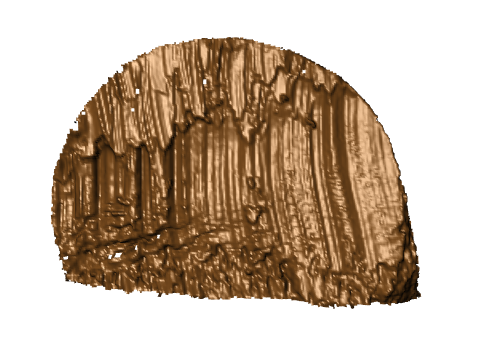
\includegraphics[width=\textwidth,height=5.5cm]{images/T1AW-LI-R1.png}

}

\subcaption{\label{fig-T1AW-LI-R1}}

\end{minipage}%
%
\begin{minipage}{0.50\linewidth}

\centering{

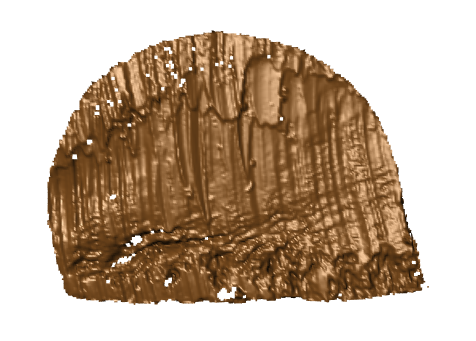
\includegraphics[width=\textwidth,height=5.5cm]{images/T2AW-LI-R1.png}

}

\subcaption{\label{fig-T2AW-LI-R1}}

\end{minipage}%
\newline
\begin{minipage}{0.05\linewidth}
~\end{minipage}%
%
\begin{minipage}{0.90\linewidth}

\centering{

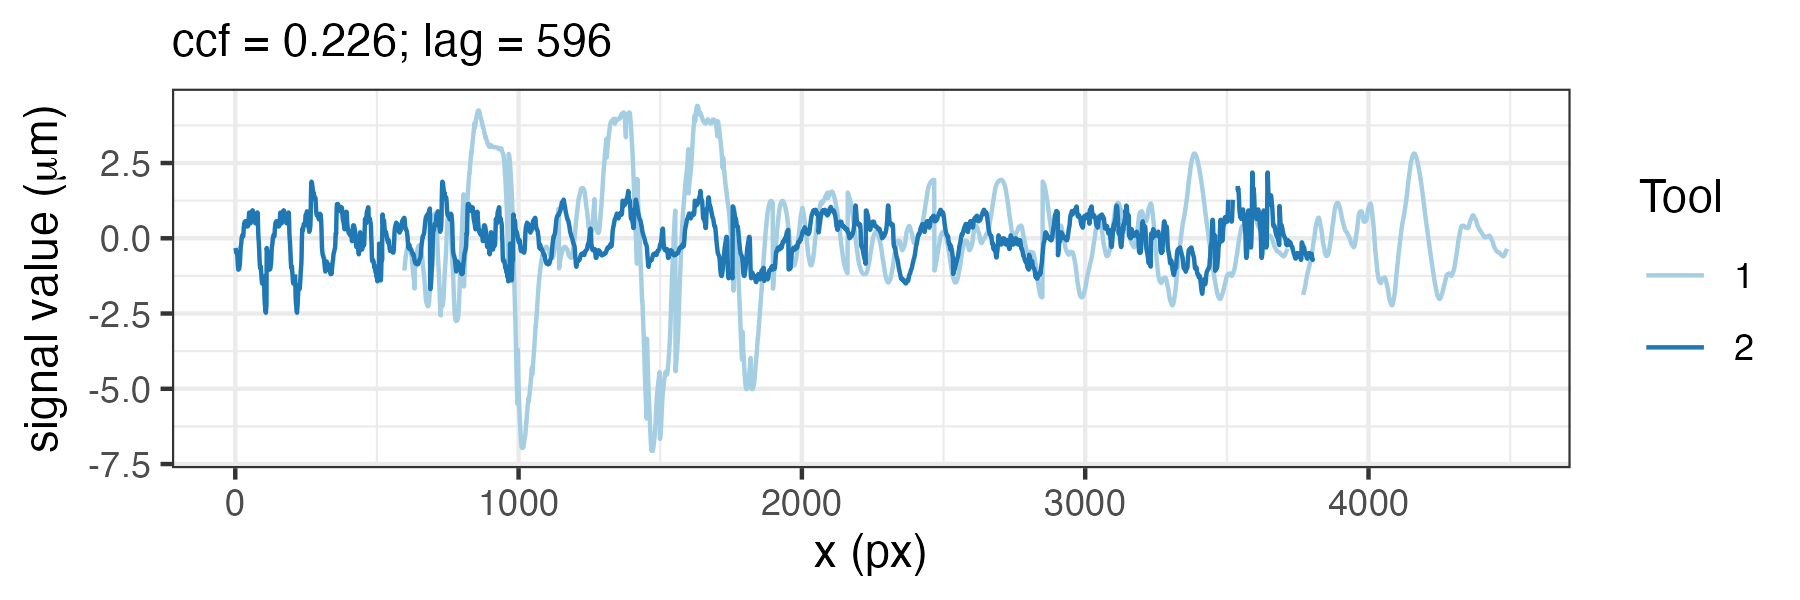
\includegraphics[width=\textwidth,height=5cm]{images/T1AW-LI-R1-T2AW-LI-R1.png}

}

\subcaption{\label{fig-T1AW-LI-R1-T2AW-LI-R1}}

\end{minipage}%

\caption{\label{fig-T1AW-LI-R1-T2AW-LI-R1-alignment}(a) Scan T1AW-LI-R1
cut by tool 1. (b) Scan T2AW-LI-R1 cut by tool 2. (c) Alignment of
signals from T1AW-LI-R1 and T2AW-LI-R1.}

\end{figure}%

\begin{figure}

\centering{

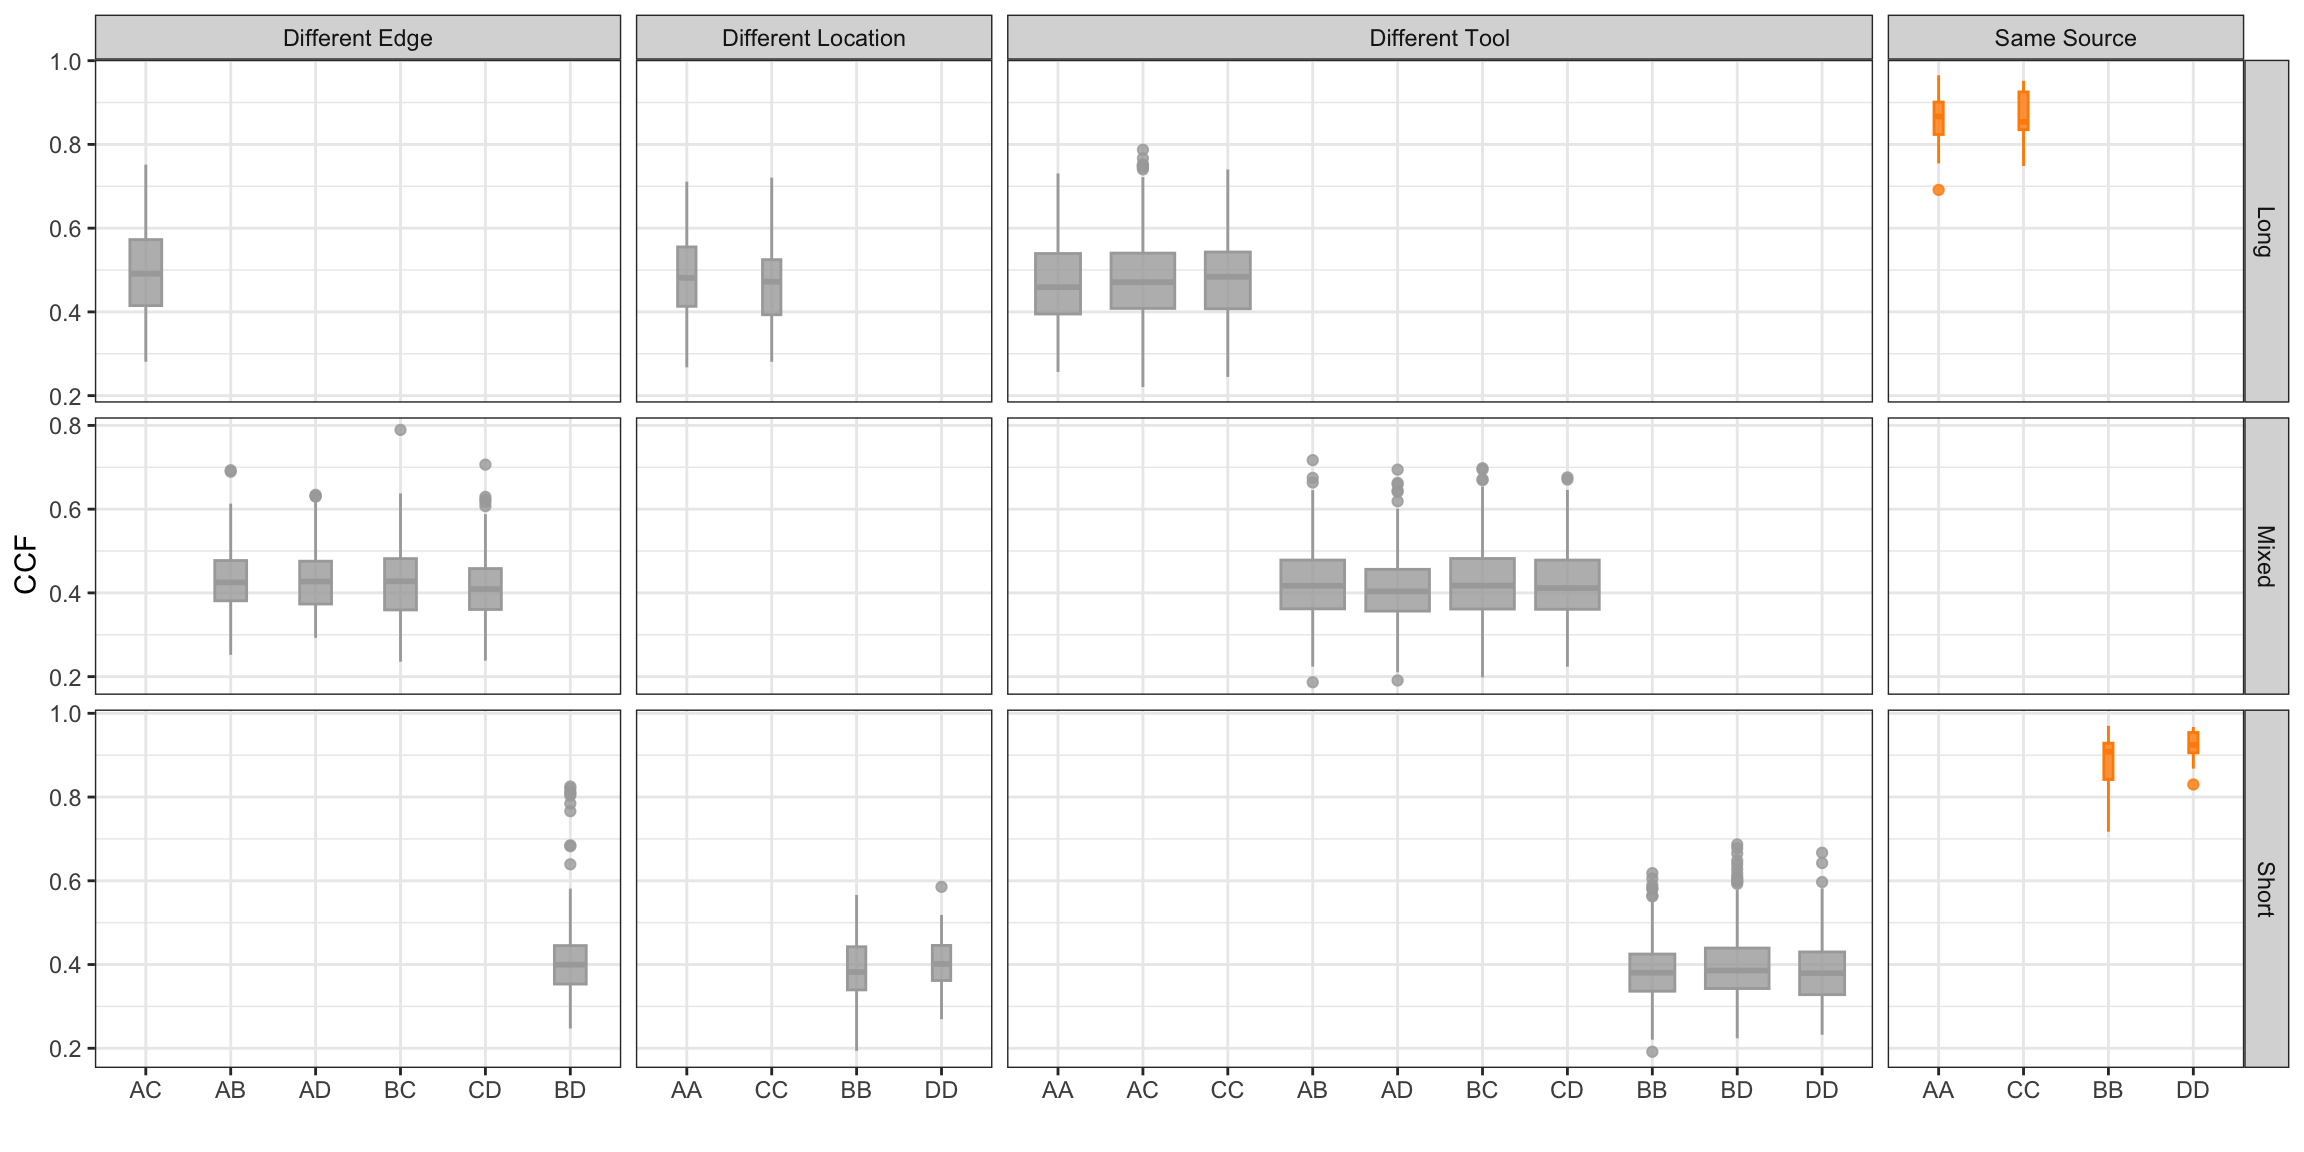
\includegraphics[width=6.77083in,height=3.125in]{images/ccf_boxplot.png}

}

\caption{\label{fig-ccf-boxplot}The boxplot shows that signals from the
same sources have higher CCfs than those from different sources.}

\end{figure}%

\begin{figure}

\centering{

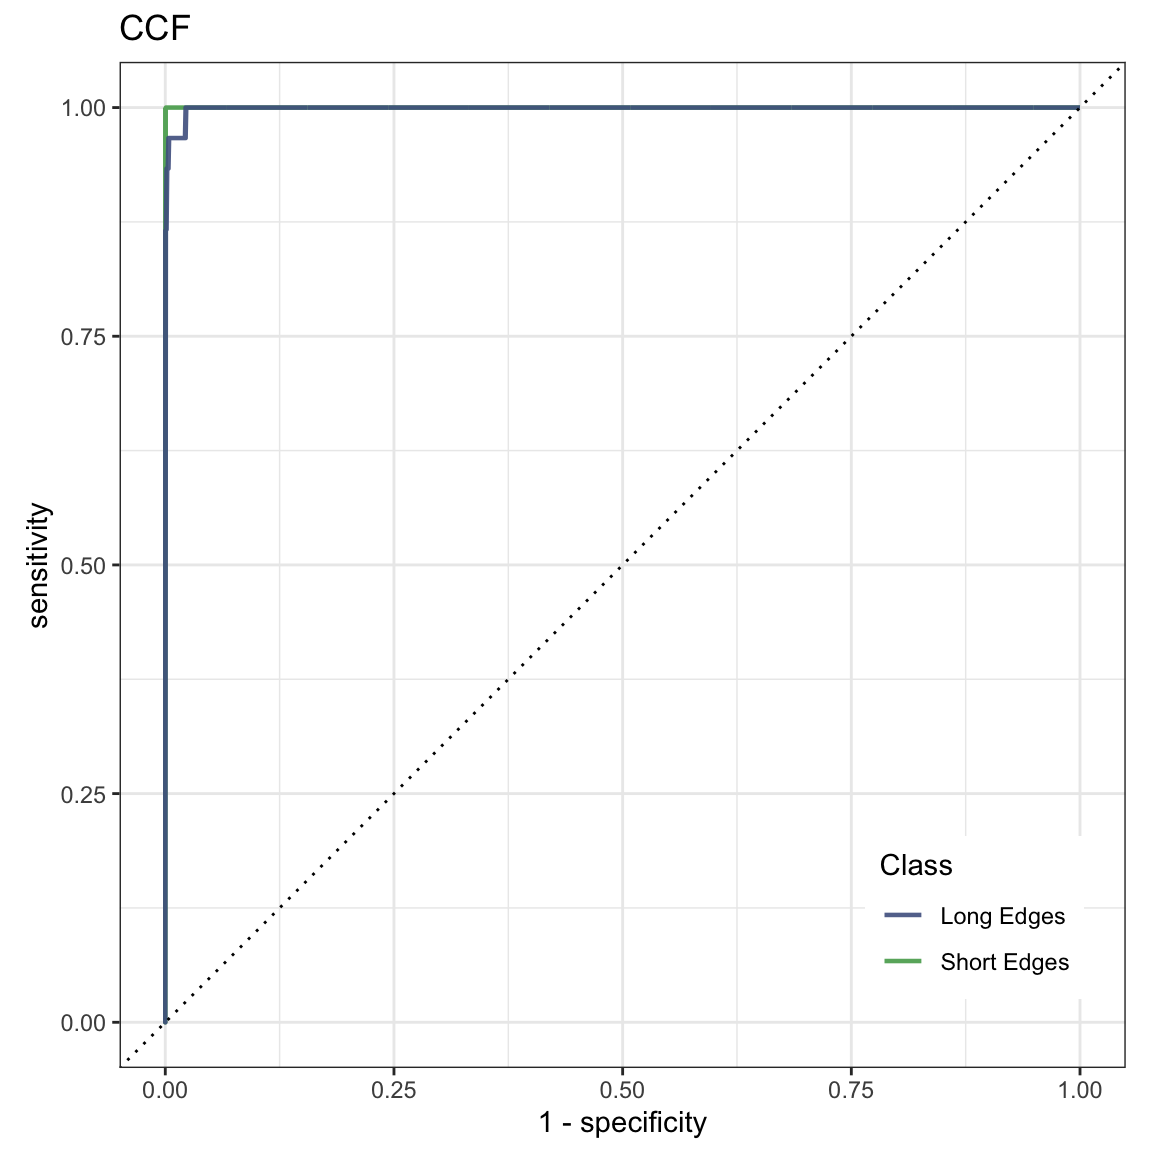
\includegraphics[width=5.20833in,height=5.20833in]{images/ccf_ROC.png}

}

\caption{\label{fig-ccf-ROC}The ROC curve is bending very close to the
upper left corner, which means excellent in classification and drawing
conclusions.}

\end{figure}%

\ifnum \ifinstruction=1

\textcolor{gray}{(unlimited length) This section presents any experiments or analyses that are needed to support the technical quality of the dataset. This section may be supported by figures and tables, as needed. This is a required section; authors must present information justifying the reliability of their data.}

\begin{itemize}
  \item
  Measurement of data quality?
  
  \begin{itemize}
    \item
    Numeric measurements / tests: ?
    
    \item
    Visualizations: ?
    
    \item
    Check with existing data: ?
    
    \item
    Questionable / slur procedures:
      
      \begin{itemize}
      \item
      \href{https://www.nature.com/articles/s41597-024-03341-w?_gl=1*5ya8g2*_up*MQ..&gclid=EAIaIQobChMInOXO84DVhgMViewWBR3vWQJAEAAYASAAEgJICfD_BwE#Sec28}{AidData’s Geospatial Global Chinese Development Finance Dataset}: \textcolor{gray}{Second, all data collected is reviewed by at least two individuals. Although this is not a double-blind review procedure, the use of satellite imagery to verify project locations results in far less uncertainty when compared to previous approaches to geocoding where locations were selected entirely based on text descriptions.}
      
      \item
      \href{https://www.nature.com/articles/s41597-024-03021-9?_gl=1*1u1zppx*_up*MQ..&gclid=EAIaIQobChMInOXO84DVhgMViewWBR3vWQJAEAAYASAAEgJICfD_BwE#Sec9}{A large open access dataset of brain metastasis 3D segmentations on MRI with clinical and imaging information}: \textcolor{gray}{A medical student (D.R.) double checked and adjusted the revised NIfTI segmentation masks and manually counted the number of lesions with contrast-enhancement, necrosis, and peritumoral edema for each patient.}
      
      \item
      \href{https://www.nature.com/articles/s41597-024-03445-3?_gl=1*1ikco52*_up*MQ..&gclid=EAIaIQobChMInOXO84DVhgMViewWBR3vWQJAEAAYASAAEgJICfD_BwE#Sec11}{Time series of freshwater macroinvertebrate abundances and site characteristics of European streams and rivers}: \textcolor{gray}{Technical validation of the TREAM dataset was achieved through exclusion of time series data that did not match our inclusion criteria and data standardisation steps (outlined in Methods above). Any noted issues that did not adhere to the outlined standardisation within the datasets from the 41 independent projects included in this dataset were checked with data providers and corrected or removed when standardisation was not achievable (e.g., when collection methods changed over the course of the time series).}
      
      \item
      \href{https://www.nature.com/articles/s41597-023-02684-0?_gl=1*1t69zgo*_up*MQ..&gclid=EAIaIQobChMInOXO84DVhgMViewWBR3vWQJAEAAYASAAEgJICfD_BwE#Sec12}{3D surgical instrument collection for computer vision and extended reality}: \textcolor{gray}{The main issue...Since we store our models in a standard format (STL), they are compatible with a large variety of visualisation and processing software.}
      
      \item
      \href{https://www.nature.com/articles/s41597-024-03396-9?_gl=1*1ikco52*_up*MQ..&gclid=EAIaIQobChMInOXO84DVhgMViewWBR3vWQJAEAAYASAAEgJICfD_BwE#Sec4}{Three-dimensional reconstruction of high latitude bamboo coral via X-ray microfocus Computed Tomography
}: \textcolor{gray}{Regular quality assurance inspections are carried out on the µ-CT scanner to verify its metrological and geometrical (alignments) accuracy for conducting the scans. The geometry of source to object and source to detector distances are verified whenever there is any significant physical interaction with the source such as re-alignment, change of filament, or source anode change. This calibration process involves scanning a specially designed phantom known as an ‘hourglass’36, which consists of three pairs of high-sphericity spheres. The sphere sizes are as follows: two spheres with a diameter of 3.000 mm, two spheres with a diameter of 6.000 mm, and two spheres with a diameter of 9.525 mm, and each sphere is kept in contact with its size-counterpart. By using this phantom, it becomes possible to accurately determine a known distance, specifically the centre-to-centre distance of the spheres, in a threshold-independent manner. If the measured distance deviates beyond the acceptable limits of metrological accuracy, the system’s calibration parameters are adjusted to ensure agreement between the measured distance and the actual distance.}
      
      \end{itemize}
      
    \end{itemize}
  
\end{itemize}
\fi

\section*{Usage Notes}\label{sec-usage-notes}
\addcontentsline{toc}{section}{Usage Notes}

The \texttt{R} package
\texttt{x3ptools}\citep{hofmannX3ptoolsToolsWorking2018} available from
\texttt{CRAN} supports working with files in \texttt{x3p} format. The
sample scripts in \texttt{R} for processing scans from \texttt{x3p}
format to their signal and alignment are available on \texttt{GitHub}
\href{https://github.com/heike/wirecuts-data}{heike/wirecuts-data} in
the \texttt{assessment/code} folder, as described in
Table~\ref{tbl-code-overview}.

\begin{table}

\caption{\label{tbl-code-overview}Overview of available codes.}

\centering{

\fontsize{12.0pt}{14.4pt}\selectfont
\begin{tabular*}{0.95\linewidth}{@{\extracolsep{\fill}}>{\raggedright\arraybackslash}p{\dimexpr 0.522\linewidth -2\tabcolsep-1.5\arrayrulewidth}|>{\raggedright\arraybackslash}p{\dimexpr 0.283\linewidth -2\tabcolsep-1.5\arrayrulewidth}>{\raggedright\arraybackslash}p{\dimexpr 0.438\linewidth -2\tabcolsep-1.5\arrayrulewidth}}
\toprule
 & Description & Section \\ 
\midrule\addlinespace[2.5pt]
\multicolumn{3}{>{\raggedright\arraybackslash}m{0.95\linewidth}}{Inspect raw scans} \\[2.5pt] 
\midrule\addlinespace[2.5pt]
\texttt{1-create\_pngs\_from\_x3p.R} & obtain images of \texttt{x3p}s in \texttt{scans/} & \protect\hyperref[sec-cutting-wires]{Cutting Wires} \\ 
\midrule\addlinespace[2.5pt]
\multicolumn{3}{>{\raggedright\arraybackslash}m{0.95\linewidth}}{Extract profiles} \\[2.5pt] 
\midrule\addlinespace[2.5pt]
\texttt{2-create\_profiles\_from\_x3p.R} & manually extract profiles from each scan & \protect\hyperref[sec-extract-profiles]{Extract Profiles} \\ 
\texttt{3-create-single-profile-file.R} & create meta profile information & \protect\hyperref[sec-extract-profiles]{Extract Profiles} \\ 
\midrule\addlinespace[2.5pt]
\multicolumn{3}{>{\raggedright\arraybackslash}m{0.95\linewidth}}{Derive signals} \\[2.5pt] 
\midrule\addlinespace[2.5pt]
\texttt{4-create\_signals\_from\_profiles.R} & derive signals from each profile & \protect\hyperref[sec-filtered-signals]{Filtered Signals} \\ 
\midrule\addlinespace[2.5pt]
\multicolumn{3}{>{\raggedright\arraybackslash}m{0.95\linewidth}}{Align signals} \\[2.5pt] 
\midrule\addlinespace[2.5pt]
\texttt{5-create-images.R} & create images for pairwise alignment & \protect\hyperref[sec-align-signals]{Align Signals} \\ 
\texttt{6-align-pairwise.R} & compute pairwise alignment CCF values & \protect\hyperref[sec-align-signals]{Align Signals} \\ 
\texttt{7-all-comparison-results.R} & visualize comparison results & \protect\hyperref[sec-align-signals]{Align Signals} \\ 
\bottomrule
\end{tabular*}

}

\end{table}%

We already conduct pairwise comparisons and visualize some of the
comparison results in \hyperref[sec-align-signals]{Align Signals} and
\hyperref[sec-technical-validation]{Technical Validation}, and we can
also produce other analysis plots.

Suppose we put the CCF values in a tilemap with different tools,
locations and edge combinations. In that case, we expect only the
diagonal to have high CCF values, close to 1 and marked as orange in the
tilemap, as the diagonal represents the same source, and the rest of the
matrix to have low CCF values, close to 0 and marked as gray. In Figure
\ref{fig-ccf-tilemap}, the behavior is consistent with our expectation
overall, except for some rare cases with tool 5 edge D. The density plot
in Figure \ref{fig-ccf-density} shows the distribution of the CCF values
with the same sources and different sources. The overlapping points
between the tails of these two distributions can be a rough threshold.

Furthermore, the ROC curve in Figure \ref{fig-ccf-ROC} shows the
sensitivity / true positive rate against the false positive rate (FPR)
(1 - specificity). The curve is very close to the upper left corner,
which is excellent for classification and drawing conclusions. It gives
us a true threshold of 0.589 to control the FPR to be less than 0.05
with a false negative rate (FNR) to be 0,
\tom{(false positive rate (FPR) / false discovery rate (FDR) -> define the H0 or call it false identification rate (FIR)???)},
and 0.658 to control the FPR to be less than 0.01, with FNR to be 0.02.

\begin{figure}

\centering{

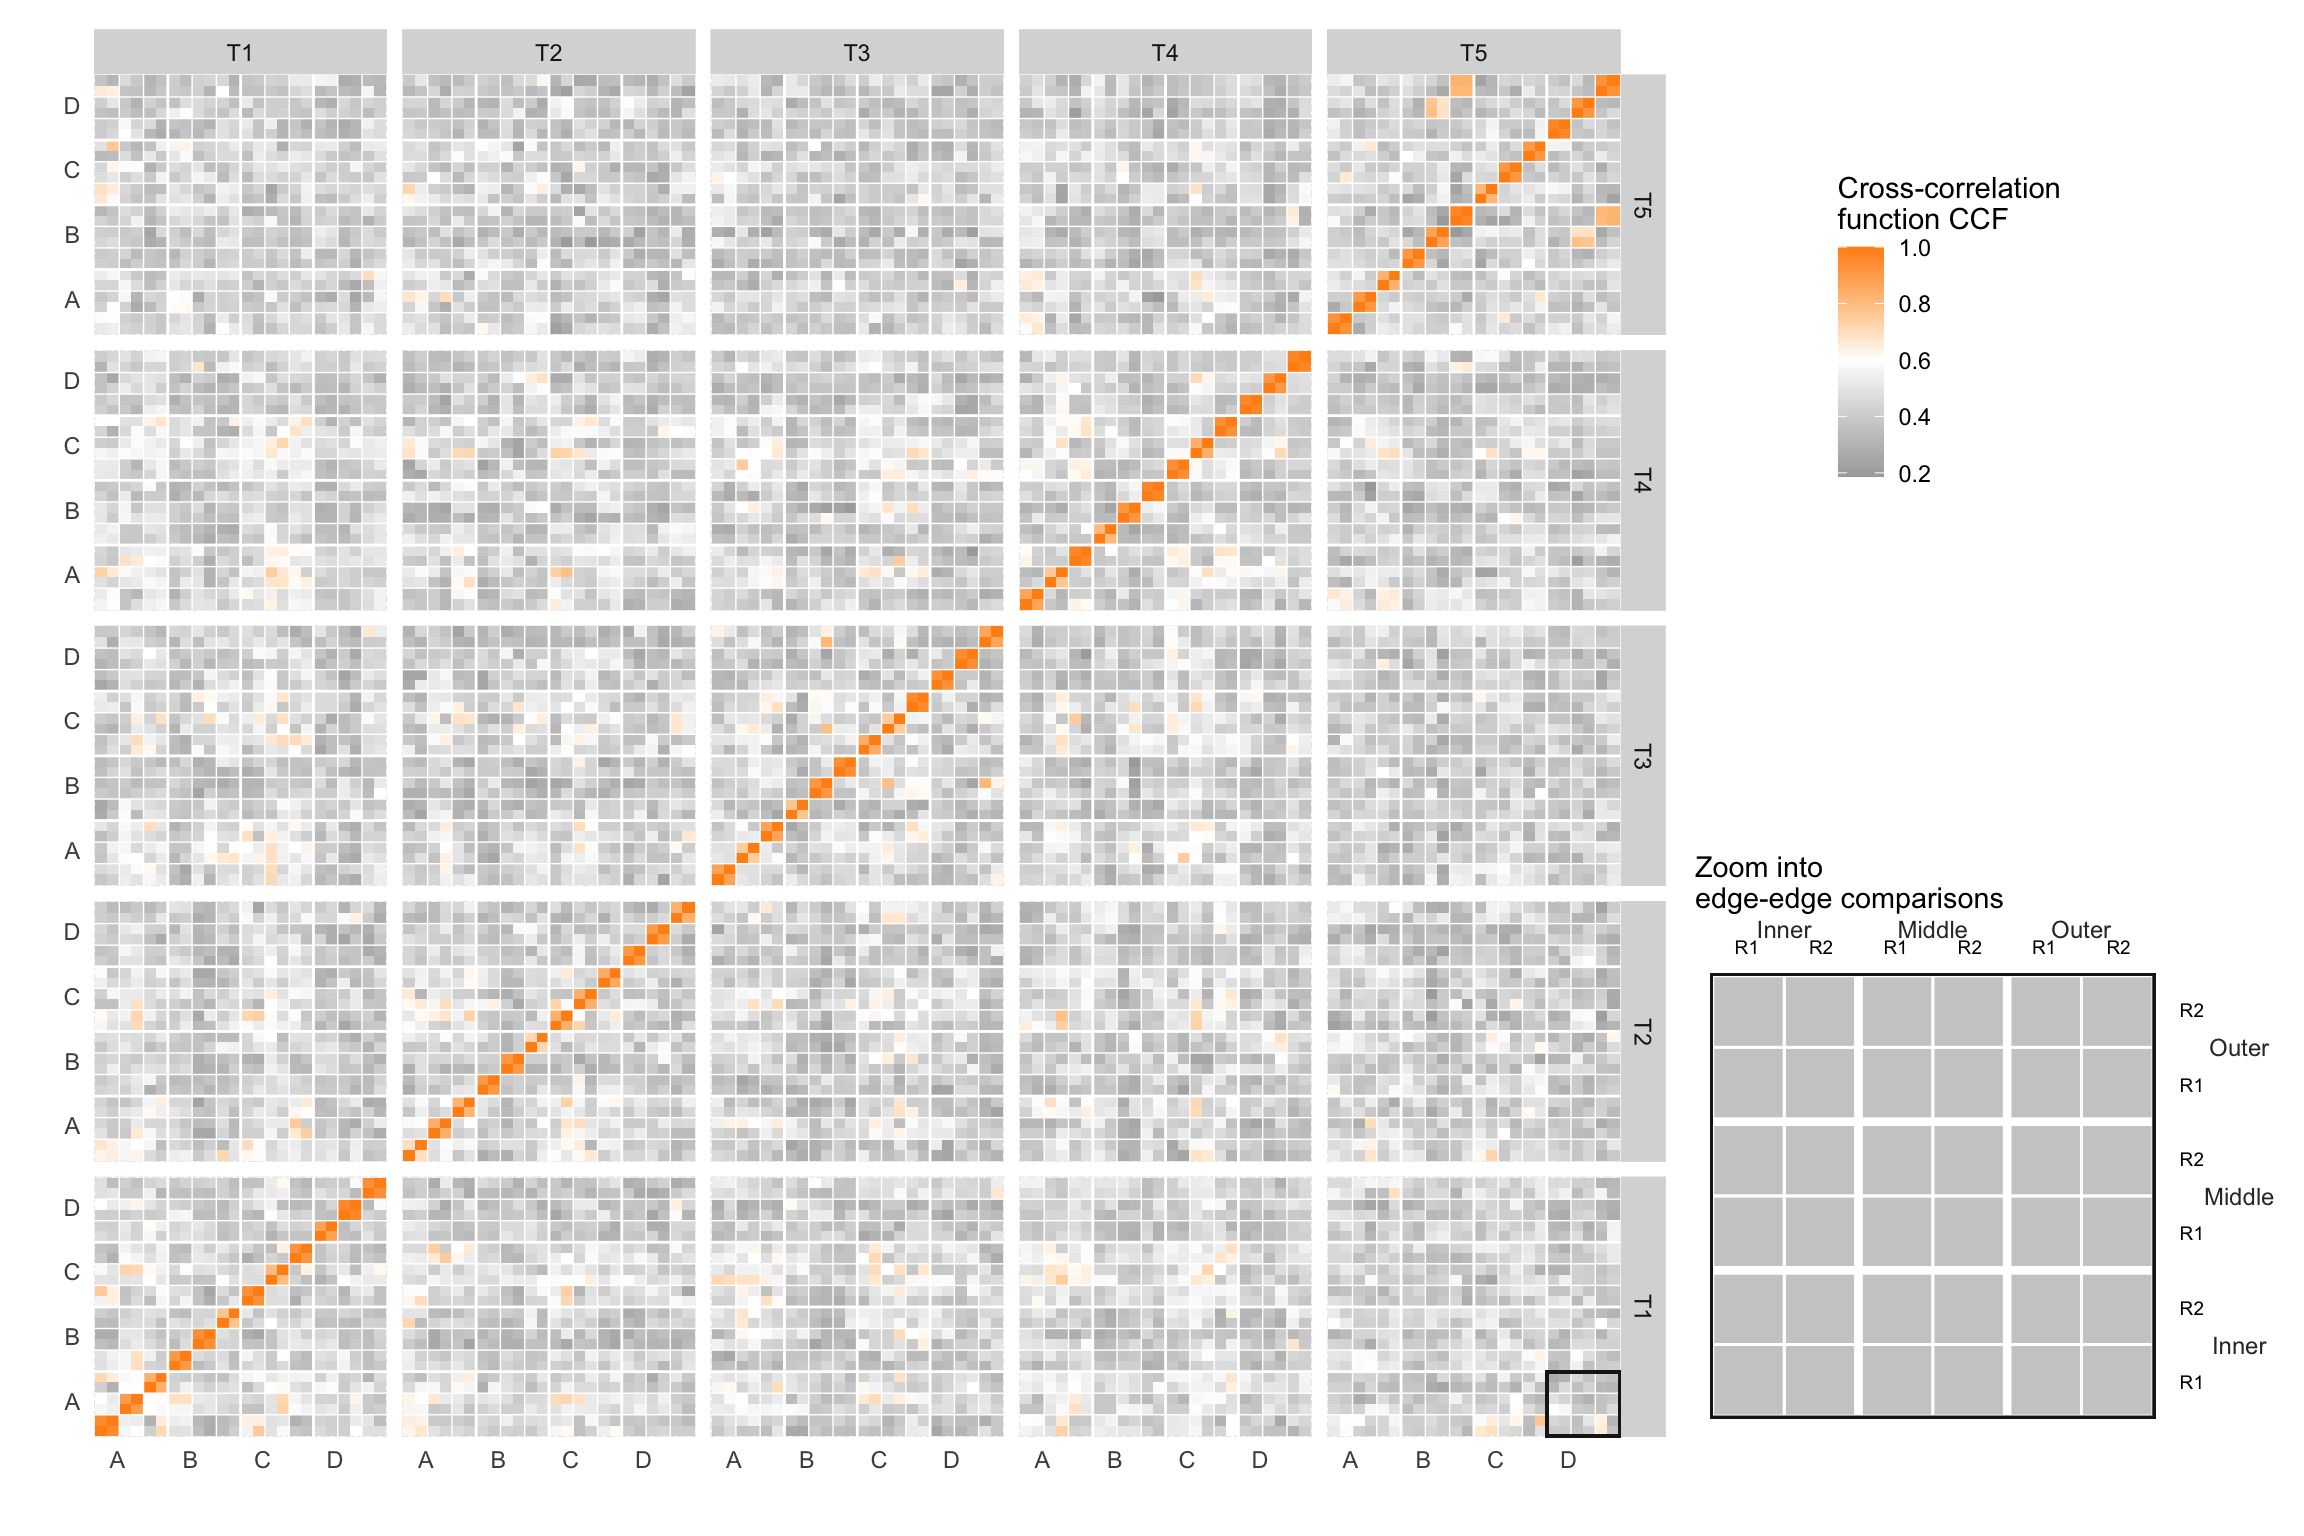
\includegraphics[width=6.25in,height=4.16667in]{images/ccf_tilemap.png}

}

\caption{\label{fig-ccf-tilemap}The tilemap shows signals from the same
source have CCFs close to 1.}

\end{figure}%

\begin{figure}

\centering{

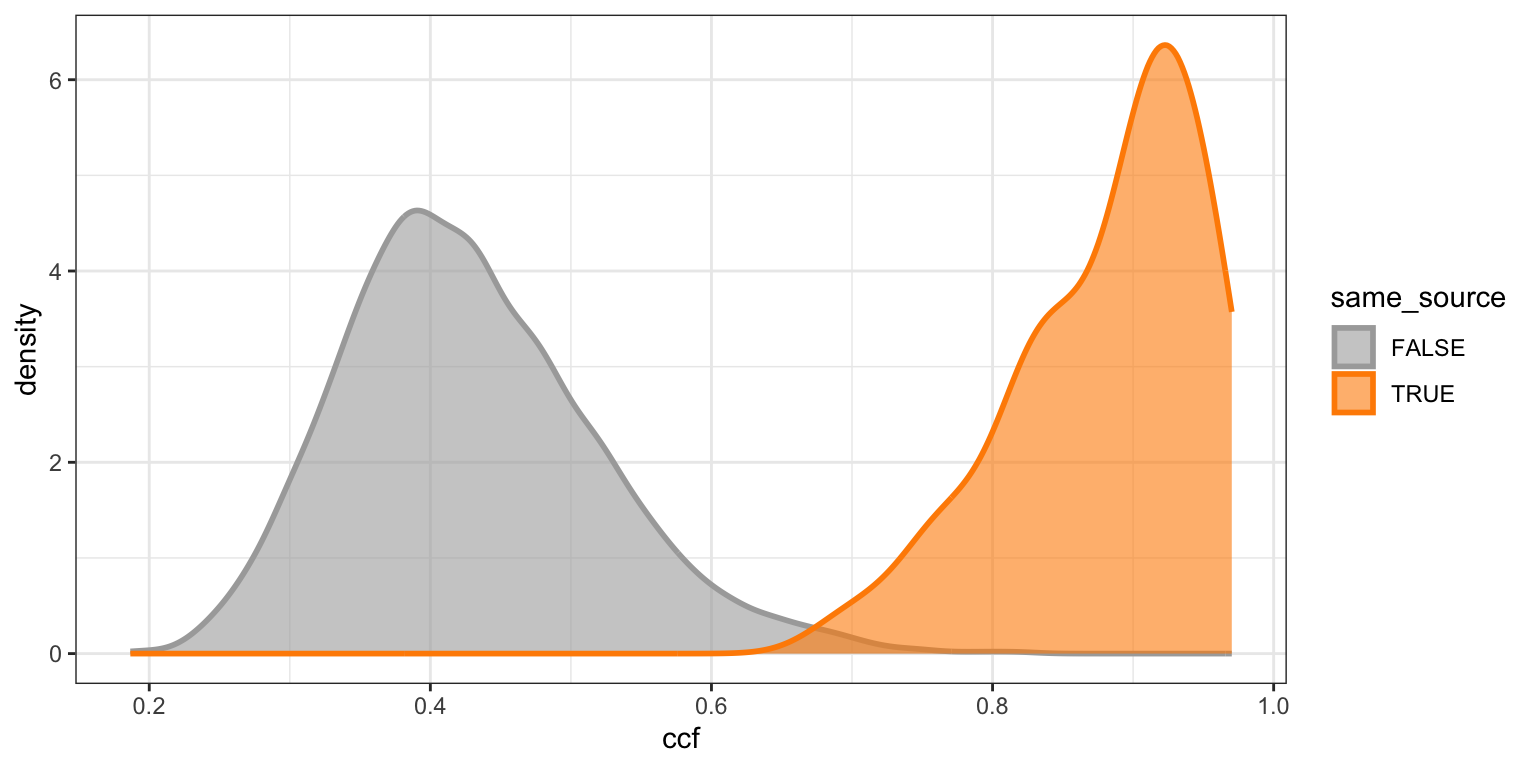
\includegraphics[width=5.20833in,height=2.60417in]{images/ccf_density.png}

}

\caption{\label{fig-ccf-density}The density plot shows tails of
distributions overlap, which can be used as a rough threshold for
drawing conclusions.}

\end{figure}%

\ifnum \ifinstruction=1

\textcolor{gray}{(unlimited length) The Usage Notes should contain brief instructions to assist other researchers with reuse of the data. This may include discussion of software packages that are suitable for analysing the assay data files, suggested downstream processing steps (e.g. normalization, etc.), or tips for integrating or comparing the data records with other datasets. Authors are encouraged to provide code, programs or data-processing workflows if they may help others understand or use the data. Please see our code availability policy for advice on supplying custom code alongside Data Descriptor manuscripts.}

\textcolor{gray}{For studies involving privacy or safety controls on public access to the data, this section should describe in detail these controls, including how authors can apply to access the data, what criteria will be used to determine who may access the data, and any limitations on data use.}
\fi

\section*{Code availability}\label{sec-code-availability}
\addcontentsline{toc}{section}{Code availability}

We made available all codes we used for inspecting raw scans, extracting
profiles, derving signals, aligning signals, and visualizing comparison
results discussed in \hyperref[sec-methods]{Methods} and
\hyperref[sec-technical-validation]{Technical Validation}, as described
in Table~\ref{tbl-code-overview}. All results are reproducible using
these codes provided.

\ifnum \ifinstruction=1

\textcolor{gray}{For all studies using custom code in the generation or processing of datasets, a statement must be included under the heading "Code availability", indicating whether and how the code can be accessed, including any restrictions to access. This section should also include information on the versions of any software used, if relevant, and any specific variables or parameters used to generate, test, or process the current dataset.}
\fi

\bibliography{references}

%\noindent LaTeX formats citations and references automatically using the bibliography records in your .bib file, which you can edit via the project menu. Use the cite command for an inline citation, %e.g. \cite{Kaufman2020, Figueredo:2009dg, Babichev2002, behringer2014manipulating}. 
%For data citations of datasets uploaded to e.g. \emph{figshare}, please use the \verb|howpublished| option in the bib entry to specify the platform and the link, as in the \verb|Hao:gidmaps:2014| example in the sample bibliography file. For journal articles, DOIs should be included for works in press that do not yet have volume or page numbers. For other journal articles, DOIs should be included uniformly for all articles or not at all. We recommend that you encode all DOIs in your bibtex database as full URLs, e.g. https://doi.org/10.1007/s12110-009-9068-2.

\section*{Acknowledgements} 
This work was partially funded by the Center for Statistics and
Applications in Forensic Evidence (CSAFE) through Cooperative Agreement
70NANB20H019 between NIST and Iowa State University, which includes
activities carried out at Carnegie Mellon University, Duke University,
University of California Irvine, University of Virginia, West Virginia
University, University of Pennsylvania, Swarthmore College and the
University of Nebraska-Lincoln.

\section*{Author contributions statement}

\hh{Let's follow the Elsevier definitions: https://www.elsevier.com/researcher/author/policies-and-guidelines/credit-author-statement}

Y.L.: Methodology, Software, Validation, Data Curation, Writing - Draft;
H.H.: Conceptualization, Methodology, Validation, Writing - Review \&
Editing; C.M.: Lab supervision; E.A.: Physical Specimen, Scanning; J.S:
Forensic advice; A.C.: Funding acquisition.
%Must include all authors, identified by initials, for example:
%A.A. conceived the experiment(s), A.A. and B.A. conducted the experiment(s), C.A. and D.A. analysed the results.

\noindent
All authors reviewed the manuscript. 

\section*{Competing interests} (mandatory statement)

H.H. is a technical advisor to AFTE (Association of Firearms and
Toolmarks Examiners), fellow of the ASA (American Statistical
Association), and committee member of the ASA Forensic Science
Committee. H.H. has testified as court witness on behalf of judge April
Neubauer, NY State Supreme Court Criminal Term in New York City.
\hh{other competing interests - Alicia?}

% XXX Delete the section below later
% \ifnum \ifinstruction=1
% \section*{Figures \& Tables}
% 
% 
% Figures, tables, and their legends, should be included at the end of the document. Figures and tables can be referenced in \LaTeX{} using the ref command, e.g. Figure \ref{fig:stream} and Table \ref{tab:example}. 
% 
% Authors are encouraged to provide one or more tables that provide basic information on the main ‘inputs’ to the study (e.g. samples, participants, or information sources) and the main data outputs of the study. Tables in the manuscript should generally not be used to present primary data (i.e. measurements). Tables containing primary data should be submitted to an appropriate data repository.
% 
% Tables may be provided within the \LaTeX{} document or as separate files (tab-delimited text or Excel files). Legends, where needed, should be included here. Generally, a Data Descriptor should have fewer than ten Tables, but more may be allowed when needed. Tables may be of any size, but only Tables which fit onto a single printed page will be included in the PDF version of the article (up to a maximum of three). 
% 
% Due to typesetting constraints, tables that do not fit onto a single A4 page cannot be included in the PDF version of the article and will be made available in the online version only. Any such tables must be labelled in the text as ‘Online-only’ tables and numbered separately from the main table list e.g. ‘Table 1, Table 2, Online-only Table 1’ etc.
% 
% \begin{figure}[ht]
% \centering
% 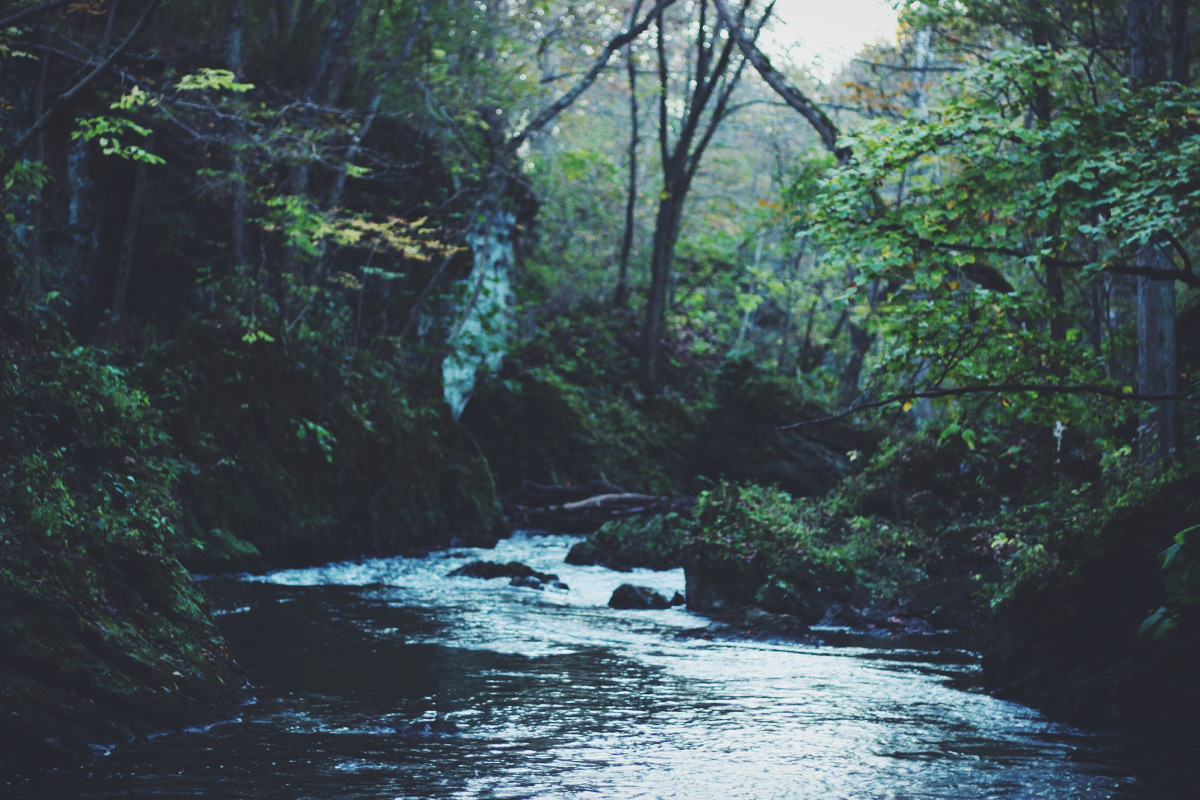
\includegraphics[width=\linewidth]{stream}
% \caption{Legend (350 words max). Example legend text.}
% \label{fig:stream}
% \end{figure}
% 
% \begin{table}[ht]
% \centering
% \begin{tabular}{|l|l|l|}
% \hline
% Condition & n & p \\
% \hline
% A & 5 & 0.1 \\
% \hline
% B & 10 & 0.01 \\
% \hline
% \end{tabular}
% \caption{\label{tab:example}Legend (350 words max). Example legend text.}
% \end{table}
% \fi

\end{document}
